\documentclass[12pt,oneside]{uhthesis}
\usepackage{subfigure}
\usepackage[ruled,lined,linesnumbered,titlenumbered,algochapter,spanish,onelanguage]{algorithm2e}
\usepackage{amsmath}
% \usepackage{amsthm}
\usepackage{amssymb}
\usepackage{amsbsy}
\usepackage{caption,booktabs}
\captionsetup{ justification = centering }
%\usepackage{mathpazo}
\usepackage{float}
\usepackage{graphicx}
\setlength{\marginparwidth}{2cm}
\usepackage{todonotes}
\usepackage{listings}
\usepackage{xcolor}
\usepackage{multicol}
\usepackage{graphicx}
\floatstyle{plaintop}
% \restylefloat{table}
\addbibresource{Bibliography.bib}
% \setlength{\parskip}{\baselineskip}%
\renewcommand{\tablename}{Tabla}
\renewcommand{\listalgorithmcfname}{Índice de Algoritmos}
%\dontprintsemicolon
\SetAlgoNoEnd

\definecolor{codegreen}{rgb}{0,0.6,0}
\definecolor{codegray}{rgb}{0.5,0.5,0.5}
\definecolor{codepurple}{rgb}{0.58,0,0.82}
\definecolor{backcolour}{rgb}{0.95,0.95,0.92}

\lstdefinestyle{mystyle}{
    backgroundcolor=\color{backcolour},   
    commentstyle=\color{codegreen},
    keywordstyle=\color{purple},
    numberstyle=\tiny\color{codegray},
    stringstyle=\color{codepurple},
    basicstyle=\ttfamily\footnotesize,
    breakatwhitespace=false,         
    breaklines=true,                 
    captionpos=b,                    
    keepspaces=true,                 
    numbers=left,                    
    numbersep=5pt,                  
    showspaces=false,                
    showstringspaces=false,
    showtabs=false,                  
    tabsize=4
}

\lstset{style=mystyle}

\title{Optimización Multiobjetivo para Sistemas AutoML}
\author{\\\vspace{0.25cm}Rodrigo Daniel Pino Trueba}
\advisor{\\\vspace{0.25cm}Dra. Suilan Est\'evez Velarde\\\vspace{0.2cm}Lic. Daniel Vald\'es P\'erez}
\degree{Licenciado en Ciencia de la Computación}
\faculty{Facultad de Matemática y Computación}
\date{Fecha\\\vspace{0.25cm}\href{https://github.com/rodrigo-pino/Thesis}{github.com/rodrigo-pino/Thesis}}
\logo{Graphics/uhlogo}
\makenomenclature

\renewcommand{\vec}[1]{\boldsymbol{#1}}
\newcommand{\diff}[1]{\ensuremath{\mathrm{d}#1}}
\newcommand{\me}[1]{\mathrm{e}^{#1}}
\newcommand{\pf}{\mathfrak{p}}
\newcommand{\qf}{\mathfrak{q}}
%\newcommand{\kf}{\mathfrak{k}}
\newcommand{\kt}{\mathtt{k}}
\newcommand{\mf}{\mathfrak{m}}
\newcommand{\hf}{\mathfrak{h}}
\newcommand{\fac}{\mathrm{fac}}
\newcommand{\maxx}[1]{\max\left\{ #1 \right\} }
\newcommand{\minn}[1]{\min\left\{ #1 \right\} }
\newcommand{\lldpcf}{1.25}
\newcommand{\nnorm}[1]{\left\lvert #1 \right\rvert }
\renewcommand{\lstlistingname}{Ejemplo de código}
\renewcommand{\lstlistlistingname}{Ejemplos de código}

\newcommand*\wildcard[2][5cm]{%
  \mbox{%
    \vbox to 3cm{%
      \vfill
      \hbox to #1{\hrulefill}\par
      \hbox to #1{\strut\hfil#2\hfil}
    }
  }
}

\begin{document}

\frontmatter
\maketitle

\begin{dedication}
    A mi madre, 

    el pilar fundamental de mi vida.

    A mi hermano,

    mi fuente de luz eterna.

    A mi padre, 

    por ser mi escudo siempre que lo necesito.

    A mi abuela,

    por malcriarme.

    A los profes de la carrera,

    por exigirme, llev\'andome a conocer nuevas fronteras.

\end{dedication}

% \include{FrontMatter/Thanks}
\begin{opinion}
En la actualidad el Aprendizaje Automático ha llegado a todas las ramas de la industria, ayudando a resolver un gran número de problemas pero creando la necesidad de un enorme número de expertos para poder utilizar las herramientas adecuadas en cada caso.
En este escenario el AutoML propone una solución ayudando con la selección de forma automática de las mejores soluciones con el problema añadido de que incrementa
el costo computacional ya que tiene que evaluar muchas soluciones para resolver cada problema. Realizando esta tarea cada vez. El área de investigación en que incursiona el estudiante propone un enfoque para que los sistemas de AutoML resolver problemas donde las métricas de evaluación estén más cerca de los requerimientos reales.

El estudiante Rodrigo Daniel Pino en esta investigación se adentra en un tema del estado del arte de gran actualidad y para eso tuvo que utilizar conocimientos de varias asignaturas de la carrera y otros que no son parte del curriculum estandar. Su propuesta implicó la definición de problemas de aprendizaje de máquina en el contexto multiobjetivo y una experimentación con diferentes problemas donde se utilizan métricas multiobjetivo. Además implicó conocer una herramienta de AutoML nueva e incorporar su estrategia para evaluar y comparar sus resultados en la práctica.

Sus resultados resultan muy prometedores, permitiendo abrir la puerta a la optimización multiobjetivo manteniendo las ventajas del AutoML heterogéneo.
Esta mejora es considerable para una herramienta del estado del arte, que ya lograba resultados comparables a las mejores herramientas de AutoML existentes.
Más aún, las estrategias desarrolladas en esta investigación han sido aplicadas solamente a un grupo de problemas y métricas, pero pueden ser extendidos fácilmente a muchos otros.

Para poder afrontar el trabajo, el estudiante tuvo que revisar literatura científica relacionada con la temática así como soluciones existentes y bibliotecas de software que pueden ser apropiadas para su utilización. Todo ello con sentido crítico, determinando las mejores aproximaciones y también las dificultades que presentan.
Todo el trabajo fue realizado por el estudiante con una elevada constancia, capacidad de trabajo y habilidades, tanto de gestión, como de desarrollo y de investigación.
Por estas razones pedimos que le sea otorgada al estudiante  Rodrigo Daniel Pino Trueba la máxima calificación y, de esta manera, pueda obtener el título de Licenciado en Ciencia de la Computación.


\begingroup
  \centering
  \wildcard{Dra. Suilan Estévez Velarde}
  \hspace{1cm}
  \wildcard{Lic. Daniel Vald\'es P\'erez}
  \par
\endgroup
\end{opinion}

\begin{resumen}
	El problema de optimizaci\'on multiobjetivo aplicado a sistemas de Aprendizaje de M\'aquina Automatizado (AutoML) es un \'area poco explorada. Este trabajo define el problema de optimizaci\'on multiobjetivo aplicado a sistemas de AutoML y propone una soluci\'on para cualquier tipo de sistema AutoML.
    Aprovechando los dos espacios sobre los que trabajan los sistemas AutoML: el espacio de b\'usqueda $\mathcal{X}$ donde se encuentran las soluciones del sistema y el espacio objetivo $\mathcal{Y}$ donde reside la evaluaci\'on de dichas soluciones respecto a ciertas m\'etricas. El sistema AutoML  genera las soluciones en $\mathcal{X}$ y las eval\'ua obteniendo un representaci\'on de cada una en $\mathcal{Y}$. El algoritmo multiobjetivo  ordena las soluciones seg\'un se evaluaci\'on en $\mathcal{Y}$.
    La propuesta se inspira en NSGA-II como algoritmo multiobjetivo para seleccionar las mejores soluciones. 
    Se realiza una implementaci\'on en AutoGOAL, un sistema orientado a resolver el problema de AutoML Heterog\'eneo.
    Se eval\'ua midiendo \textit{f-score} contra tiempo de entrenamiento y precisi\'on contra recobrando obteniendo resultados satisfactorios. 
    %que prueban la adici\'on de optimizaci\'on multiobjetivo a sistemas AutoML un beneficio inmediato.

\end{resumen}

\begin{abstract}
    Multiobjective optimization applied to Automated Machine Learning (AutoML) systems is an underexplored research area. This project defines the optimization problem of multiple criteria applied to AutoML systems. It proposes a generalized solution that can be applied to any type of AutoML system by taking advantage of the two spaces where AutoML framework operates: the decision space $\mathcal{X}$ where solutions are located and the objective space $\mathcal{Y}$ where the solution's evaluations are found. The AutoML system manages pipeline generation and evalutaion so that every solution has it's own representation in $\mathcal{Y}$ where the multiobjective algorithm selects the top solutions. An adaptation of NSGA-II is used as the multiobjective algorithm. An implementation is done on top of AutoGOAL, a system which targets the Heterogeneus AutoML problem. Tests are done with f-score versus training time and precision versus recall having satisfactory outcomes.
\end{abstract}

\tableofcontents
\listoffigures
% \listoftables
\listofalgorithms
% \lstlistoflistings


\mainmatter

\chapter*{Introducción}\label{chapter:introduction}
\addcontentsline{toc}{chapter}{Introducción}
La sociedad moderna est\'a cada vez m\'as digitalizada donde algoritmos de inteligencia artificial se integran progresiva y gradualmente a nuestras vidas. En la medicina para la predicci\'on de enfermedades como el c\'ancer \brackcite{kourou2015machine}, las noticias  recomendadas basadas en nuestros gustos online \brackcite{liu2010personalized}, los carros inteligentes que se conducen a s\'i mismos con m\'inima interacci\'on por parte del piloto \brackcite{badue2021self}, detecci\'on de sentimientos de odio en un texto \brackcite{fortuna2018survey} e incluso en el arte, donde sistemas producen im\'agenes partiendo de descripciones textuales \brackcite{xu2018attngan}.

El Aprendizaje Autom\'atico (\textit{Machine Learning} en ingl\'es) es una rama de la inteligencia artificial que compone el n\'ucleo de estas aplicaciones, no obstante, el n\'umero de expertos disponibles sobre el tema no es suficiente para la creciente demanda de programas de este tipo. Los modelos o flujos de aprendizaje de m\'aquina requieren para su correcto funcionamiento de un buen dise\~no determinado por la selecci\'on de t\'ecnicas de aprendizaje e hiperpar\'ametros que lo componen. 
La modelaci\'on  es una tarea que requiere conocimientos, experiencia y abundante prueba y error.
% TODO: Mejorar escritura, cual es la insuficiencia  no queda claro
Con el objetivo de mitigar est\'a insuficiencia nace el Aprendizaje de M\'aquina Automatizado, una l\'inea de investigaci\'on dirigida a automatizar esta parte del proceso.

Los programas que resuelven el problema de Aprendizaje Automatizado son conocidos como sistemas AutoML y var\'ian en la parte de trabajo del experto que desean automatizar: desde la selecci\'on autom\'atica de hiperpar\'ametros \brackcite{feurer2019hyperparameter} a la selecci\'on de modelos \brackcite{thornton2013auto} o ambos  simult\'aneamente. El objetivo general de estos sistemas es producir una selecci\'on tal que el modelo final maximice  respecto a cierta m\'etrica o criterio de evaluaci\'on. 
% TODO: Esta oracion necesita cita?
Usualmente esta m\'etrica representa la relevancia de los resultados obtenidos.

En el contexto actual, existen problemas para los cuales ya no es suficiente que un modelo de Aprendizaje Autom\'atico obtenga resultados relevantes pues se requiere adem\'as un buen desempe\~no respecto a criterios adicionales. En el campo del Aprendizaje de M\'aquina Automatizado esto implica la necesidad de incrementar la expresividad para describir los problemas con tal de obtener mayor control sobre las soluciones que estos generan. Entre las propuestas para lograr esto se encuentra la adici\'on de optimizaci\'on simult\'anea de m\'ultiples criterios de evaluaci\'on a los sistemas AutoML  tal que los modelos de Aprendizaje Autom\'atico producidos tengan buen rendimiento en estos.   

\section*{Motivaci\'on}
% Los modelos de Aprendizaje de M\'aquina forman cada vez m\'as y m\'as parte de la vida diaria, aplic\'andose en situaciones directamente  relacionadas con la vida de los seres humanos. 
% TODO: Reescribir este parrafo para que se entienda que se sigue hablando de Multiobjetivo, y de xq es imortante
Un problema conocido y estudiado es el sesgo en los flujos de Aprendizaje de M\'aquina. Existen casos donde ciertas caracter\'isticas de los datos pueden provocar que las predicciones de un modelo se encuentren parcializadas en favor de una mayor\'ia  \brackcite{mehrabi2021survey} afectando su capacidad de predicci\'on. Esto tiene mayor importancia cuando los datos representan seres humanos y la decisi\'on del modelo tiene un impacto directo o indirecto en la vida de un individuo o grupo. Se desea que el modelo no discrimine por el color de piel, g\'enero o regi\'on y a la vez sus resultados se mantengan relevantes. Es necesario entonces que el flujo sea capaz de poder optimizar tanto  relevancia como  nivel de justeza, un problema multiobjetivo.

% TODO: Poner referencia  a situaciones de interpretabilidad y de robustez
Tambi\'en hay situaciones donde se desea obtener un modelo que sea relevante a la par de \textit{interpretable}, que implica entender sin necesidad de ser un experto porque el flujo toma ciertas decisiones, o cu\'an \textit{robusto} es, tal que perturbaciones en los datos de entrada no cambien radicalmente el resultado de este.

La optimizaci\'on multiobjetivo en AutoML permite el uso de m\'etricas que no tienen sentido usarlas individualemente como \textit{precisi\'on} y \textit{recobrado}. 
 \textit{Precisi\'on} mide la proporci\'on entre los valores relevantes identificados y todos los valores identificados
 mientras que \textit{recobrado} mide la proporci\'on entre los valores relevantes identificados y todos los valores relevantes.
Estas m\'etricas cuando se usan por separado no representan la relevancia de un modelo pues basta para tener un recobrado perfecto seleccionar todos los elementos del conjunto de datos, y una precisi\'on casi perfecta escogiendo un pequeño conjunto de elementos.
\textit{F-score} relaciona ambas medidas y permite el uso de  par\'ametros para priorizar una o la otra seg\'un el investigador determine. 
Un sistema AutoML Multiobjetivo puede prescindir de m\'etricas como \textit{f-score} pues es capaz de optimizar en paralelo para todos los criterios que la componen.
%que pueda realizar una b\'usqueda optimizando en paralelo para ambos criterios y obtener soluciones que representen todas las maneras de parametrizar \textit{f-score} en una solo ciclo de ejecuci\'on.
%puede producir soluciones variadas cada una representativa de ejecutar el problema con el f-score variando los parametros.


\section*{Antecedentes}
% Darle vaselina a esto:
% - Partir de que exsite un marco de trabajo respecto a sistemas AutoML: AutoGOAL 
% - Partir de que hay un estudio sobre sesgos en inteligencia artificial
% - Por ende, se quiere trabajar en una propuesta que permita multiobjetivo

% TODO: Es necesario especificar a que colectivo me refiero
En el entorno del grupo de Inteligencia Artificial de la facultad de Matem\'aticas y Computaci\'on de la Universidad de La Habana se desarrolla diversas l\'ineas de investigaci\'on centradas en el Aprendizaje de M\'aquina Automatizado. AutoGOAL \brackcite{estevez2020solving} es una herramienta creada por el colectivo con el objetivo de resolver el problema AutoML Heterog\'eneo.

La entidad tambi\'en desarrolla otras l\'ineas donde se estudia la posible mitigaci\'on de sesgos en flujos producidos por sistemas AutoML \brackcite{consuegra2022intelligent}. 
%Esto requiere de poder optimizar para m\'etricas adicionales como justeza.

% Este trabajo es una propuesta que pretende incrementar la expresividad con que se pueden definir problema se AutoML. que tienen los usuarios para la b\'usqueda de sus soluciones permitendo la utilizaci\'on de varias m\'etricas.
%AutoGOAL una herramienta de AutoML que utilza algoritmos gen\'eticos y permite genera 

\section*{Problem\'atica}
% No darle la vuelta al pollo
% Decir cual es el problema: Poder utilizar optimizacion multiobjetivo dentro de AutoGOAL
Resolver el problema multiobjetivo en AutoML es un tema poco estudiado y con aplicaciones pr\'acticas en la actualidad.
Los sistemas AutoML de mayor reconocimento en el campo solo son capaces de optimizar para una sola m\'etrica. 

Los sistemas de AutoML utilizan espacios de b\'usqueda ca\'oticos y no diferenciables para los cuales se necesitan algoritmos agn\'osticos a esos espacios y resistentes a formas extra\~nas del frente de Pareto. Es necesario definir un algoritmo evolutivo multiobjetivo lo suficientemente general que resuelva el problema multiobjetivo y que sea compatible con cualquier sistema de AutoML.

% La capacidad de optimizar paralelamente para varios objetivos no resulta trivial y es necesario la integraci\'on de un algoritmo que sea lo m\'as resistente a este espacio sin sacrificar la obtenci\'on de buenos resultados. En la literatura hay varios ejemplos de optimizaci\'on multiobjetivo pero ninguno aplicado directamente al campo del AutoML. Los algoritmos evoluacionarios han resultado ser los mejores para la optimizaci\'on multiobjetivo pues cumplen con estas caracter\'isticas.

%Los sistema de Aprendizaje de M\'aquina Automatizado basados en algoritmos evolutivos son los que pueden tener el espacio de decision m\'as amplio.
%Se propone añadir multi objetivo para optimizar respecto a varias m\'etricas de evaluaci\'on simult\'aneamente. Se quiere utilizar una implementaci\'on de algoritmos gen\'etico ya que han demostrado ser los mejores en la literatura.
%Al  funcionar los dos con algoritmos evoluacionarios se busca hacer una integraci\'on entre ambos.

% \section*{Hip\'otesis}
% La integraci\'on de sistema AutoML genetico con algoritmo genetico

 
\section*{Objetivo}
\subsection*{Objetivo General}
Optimizaci\'on Multiobjetivo para sistemas AutoML
\subsection*{Objetivos Espec\'ificos}
\begin{itemize}
    \item Estudiar el estado del arte sobre sistemas de Aprendizaje de M\'aquina Automatizado
    \item Estudiar conceptos y principios de la optimizaci\'on multiobjetivo y sus aplicaciones en el campo del Aprendizaje de M\'aquina Automatizado
    \item Identificar e implementar un algoritmo multiobjetivo que aproveche la estructura de AutoGOAL y su implementaci\'on de Probabilistic Grammatic Evolution (PGE)
    \item Experimentar y analizar los resultados de aplicar AutoGOAL Multiobjetivo a problemas conocidos de la literatura.
\end{itemize}

\section*{Estructura de la Tesis}
El resto del documenta se encuentra organizado de la siguiente manera. En el cap\'itulo \ref{chapter:state-of-the-art} se estudia t\'ecinas de AutoML y optimizaci\'on multiobjetivo que conforman el estado del arte, as\'i como ejemplos de sistemas AutoML que apliquen t\'ecnicas de optimizaci\'on multiobjetivo. En el cap\'itulo \ref{chapter:proposal} se desarrolla una propuesta generalizada para resolver el problema de AutoML Heterog\'eneo utilizando optimizaci\'on multiobjetivo. El cap\'itulo \ref{chapter:implementation} muestra una implementaci\'on de la propuesta utilizando AutoGOAL. Finalmente, En el cap\'itulo \ref{chapter:experiments} se muestran resultados obtenidos tras aplicar la propuesta en tres corpus de datos distintos utilizando optimizaci\'on multiobjetivo para dos pares de m\'etricas. 
% Finalmente, en el cap\'itulo 5 se presentan las conclusiones de la investigaci\'on.

\chapter{Estado del Arte}\label{chapter:state-of-the-art}
El proceso de investigaci\'on para dise\~nar un flujo de Aprendizaje Autom\'atico requiere una experemintaci\'on variada donde se combinan m\'ultiples t\'ecnicas como redes neuronales, clasificadores supervisados, algoritmos de agrupamientos, entre otras. Adem\'as por cada selecci\'on de las anteriores se deben optimzar adecaudamente los hiperpar\'ametros que la componen.

Con el uso de un sistema AutoML el investigador ya no tiene que crear el flujo de Aprendizaje Autom\'atico manualmente y puede dedicarse a realizar otras tareas como el adecuado preprocesamiento de los datos o ingenier\'ia de caracter\'istcas, no obstante, el proceso de automatizaci\'on viene con un costo. Cuando al experto necesita m\'as que modelos que produzcan resultados relevantes los sistemas AutoML actuales se tornan insuficientes pues no posee el suficiente control para comunicarle al sistema su intenci\'on de gu\'iar la b\'usqueda en otros sentidos.
% de controlar el espacio de decsi\'on  desea un mayor control sobre los flujos producidos tal que tengan un buen desempe\~no con respecto a alguna m\'etrica adicional, los sistmeas AutoML dejan de ser de \'utiles pu\'es en el estado del arte actual del Aprendizaje Automatizado no existe el soporte para esto.

En la secci\'on \ref{background:automl} se  hace un estudio del estado del arte en AutoML. Luego en la secci\'on \ref{background:moo} se estudia los diferentes paradigmas de Optimizaci\'on Multiobjetivo y se muestran diferentes propuestas de cada uno. Finalmente en la secci\'on \ref{background:mooautoml} se analiza casos conocidos donde al problema AutoML se le ha aplicado optimizaci\'on multiobjetivo.

\section{Aprendizaje de M\'aquina Automatizado}\label{background:automl}
% Que es AutoML
El Aprendizaje de M\'aquina Automatizado (Automated Machine Learning, AutoML) consiste en la generaci\'on autom\'atica de flujos, algoritmos o par\'amteros que resuelven un problema determinado minimizando la dependencia del usuario. 

Actualmente los sistemas AutoML se pueden en separar en dos conjuntos dependiendo del problema a resolver. Se encuentran los sistemas orientados a aprendizaje profundo que proponen resolver el problema de B\'usqueda de Arquitecturas Neuronales (\textit{Neural Arquitectural Search}, NAS) y  sistemas AutoML basado en selecci\'on y combinaci\'on; este \'ultimo puede solucionar o no el problema NAS. El segundo conjunto intenta resolver el problema de combinaci\'on, selecci\'on y optimizaci\'on de hiperpar\'ametros (\textit{Combined Algorith Selection and Hyperparameter Optimization}, CASH) acuñado por Auto-Weka (\cite{thornton2013auto}). M\'as formalmente:
\begin{definition}
    Sea $A = \{a^1, ..., a^k\}$  un conjunto de algoritmos con espacios de configuraci\'on asociados $\Lambda^1, ..., \lambda^k$.
    Sea $D$ un conjunto de datos  que se divide en $\{D_{t}^{(1)},..., D_{t}^{(k)}\}$ y $\{D_{v}^{(1)},..., D_{v}^{(k)}\}$ 
    tal que $\forall i, 1 \leq i \leq k$ se cumple que $D_{t}^{(i)} = D \setminus D^{(i)}_{v}$
    El problema CASH se define como el computo de:
    \begin{equation*}
        a^*_{\lambda^*} \in argmin_{a^{(j)} \in A, \lambda \in \Lambda^{(j)}} \frac{1}{k} \sum^{k}_{i = 1}\mathcal{L}(a^(j)_\lambda, D^{(i)}_t, D^{(i)}_v)
    \end{equation*}
    Donde $\mathcal{L}(a, D_t, D_v)$ es la funci\'on de p\'erdida al ser entrenado en $D_t$ y evaluado en $D_v$.
\end{definition}


% El objetivo es transferir el problema de combinaci\'on, selcci\'on y optimizaci\'on de hiperpar\'ametros(\textit{Combined Algorithm Selection and Hyperparameter Optimization}, CASH por sus siglas en ingl\'es) del investigador al sistema, permitiendole a este enfocarse en otras tareas como la validaci\'on de los datos o ingenier\'ia de caracter\'istcas.

En el campo del Aprendizaje de M\'aquina Automatizado cuenta con numerosas propuestas de distintos dominios: 
\begin{itemize}
    \item Optimizaci\'on Bayesiana%(\cite{hutter2019automated})
    \item Programaci\'on Evolutiva%(\cite{chen2018autostacker})
    \item B\'usqueda Aleatoria 
    \item Aprendizaje por Refuerzo
    \item M\'etodo de Gradiente
    \item Modelos Constructivos
    \item Monte Carlo
\end{itemize}

\subsection{Optimizaci\'on Bayesiana}
Las propuestas basadas en optimizaci\'on bayesiana est\'an divididas en dos componentes principales: un modelo estad\'istico bayesiano para modelar la funci\'on objetivo, y una funci\'on de adquisici\'on que dirige la b\'usqueda en el espacio. Esos sistemas utilizan el modelo estad\'istico para seleccionar el mejor candidato a evaluar. Luego de la evaluaci\'on se actualiza el modelo y se repite el proceso.

\paragraph{Auto-WEKA (\cite{thornton2013auto})} Utiliza como algoritmos de aprendizaje las m\'aquinas WEKA, una popular biblioteca de Aprendizaje Autom\'atico en Java. Presenta dos optimizadores bayesianos, una propuesta de configuraci\'on secuencial de Algortimos basados en Modelos (SMAC por \cite{hutter2011sequential}) y un estimador de Parzen con estrucutra de \'arbol (TPE por \cite{bergstra2011algorithms}), ambos se ejecutan en paralelo y se retorna la funci\'on con menor error en validaci\'on de entre todas las descubiertas.

\paragraph*{Auto-skelearn (\cite{feurer2015efficient})} Utiliza como biblioteca de aprendizaje autom\'atico a scikit-learn (\cite{pedregosa2011scikit}) y extiende la propuesta de AutoWEKA  introduciendo mejoras como la inclusi\'on de un paso de meta-aprendizaje que reduce el espacio de b\'usquda aprendiendo de modelos que obtuvieron un buen desempe\~no en conjuntos de datos similares y luego un paso de selecci\'on de ensemblers que le permite reusar los flujos de Aprendizaje de M\'aquina que tuvieron mejor rendimiento. 

\paragraph*{HyperOpt-Sklearn (\cite{komer2014hyperopt})} Similar a Auto-Skelearn con respecto a la bibliteca de aprendizaje subyacente, scikit-learn, utiliza Hyperopt (\cite{bergstra2013hyperopt}) para describir el espacio de b\'usqueda. Provee una infterfaz de optimziaci\'on que distingue un espacio de configuraciones y una funci\'on de evaluaci\'on que asigna valores de p\'erdida reales a puntos dentro de dicho espacio. Hyperopt requiere que el espacio est\'e definido como una distribuci\'on de probabilidad, permitiendo una codificaci\'on m\'as expresiva de las intuiciones de los expertos con respecto a los valores de los hiperpar\'ametros. Utiliza SMBO (\textit{Sequential Model-based Bayesian Optimization}), considerando este algoritmo como una componente intercambiable con el fin de que cualquier t\'ecninca de b\'usqueda pueda ser utilizada con cualquier problema de b\'usqueda.

% TODO: Cite keras, or autokeras
\paragraph*{Auto-Keras (\cite{jin2018efficient})} Un sistema de AutoML enfocado en resolver el problema NAS. Est\'a basado en la biblioteca Keras de Python, utilizada para crear redes neuronales.  La idea prinicipal de esta propuesta es explorar el espacio mediante la transformaci\'on de redes, utilizando un algorimto de Optmizaci\'on Bayesiana eficiente. Dichas transformaciones permiten generar redes manteniendo las configuraciones alcanzadas con entrenamientos anteriores, disminuyendo el uso de los recursos de c\'omputo. Auto-Keras a nivel t\'ecnico est\'a estructurado para el uso eficiente de la memoria y la ejecuci\'on en paralelo sobre el CPU y el GPU.

\paragraph*{autogxgboost (\cite{thomas2018automatic})} Se cat\'aloga como un sistema AutoML \textit {single-learner} debido a que solo utiliza un algoritmo de aprendizaje y optimiza los hiperpar\'ametros para este utilizando optimizaci\'on bayesiana. Requiere que el algoritmo sea un metodo de aumento de gradiente con \'arboles (\textit{Gradient Boosting with Trees}, GBT) como \textit {xgboost} (\cite{chen2016xgboost}) debido a su prometedor rendimiento con los param\'etros adecuados.   
    
\subsection{Programaci\'on Evolutiva}
     Los sistemas AutoML bas\'ados en programaci\'on evolutiva funcionan creando una poblaci\'on inicial de flujos v\'alidos para luego seleccionar los de mejor rendmiento respecto a cierta m\'etrica. Los m\'as aptos son utilizados para crear la poblaci\'on de la pr\'oxima iteraci\'on. Las propuestas difieren principalmente en como modelan el espacio de b\'usqueda y que estrategias usan para crear los nuevos individuos.
     
\paragraph*{TPOT (\cite{pmlr-v64-olson_tpot_2016})} Utiliza algoritmos de aprendizaje de la biblioteca scikit-learn (\cite{pedregosa2011scikit}) junto con el algoritmo xgboost (\cite{chen2016xgboost}), es uno de los sistemas AutoML evolutivos m\'as reconocidos. Cada algoritmo de Aprendizaje Autom\'atico a su disposici\'on se le considera un operador, adem\'as de tener un operador especial de cruce. Permite tener varias copias del dataset y aplicar operadores sobre ellos simult\'aneamente para luego recombinarlos y crear flujos con los operadores que hayan tenido mejor rendimiento. TPOT adem\'as realiza una b\'usqueda multiobjetivo sobre las soluciones encontradas utilizando NSGA-II (\cite{deb2002fast}) optimzando simultaneamente la relevancia de los resultados y minimizando la cantidad de operadores aplicados sobre los flujos de Aprendizaje Autom\'atico para mantener las soluciones simples y evitar el sobreajuste a los datos.

\paragraph*{RECIPE (\cite{de2017recipe})} Utiliza programaci\'on gen\'etica basado en gram\'aticas (\textit{Grammar Genetic Programming}, GGP) para generar sus flujos. El sistema recibe como entrada un conjunto de datos y una gram\'atica libre del contexto (CFG) que utiliza para formar una poblac\'on inicial de flujos. Partiendo de los mejores individuos aplica operadores de mutaci\'on y cruce sobre estos tal que no se violen las reglas de la gram\'atica para la obtenci\'on de una nueva poblaci\'on. Utiliza como base de aprendizaje a la bibliotea scikit-Learn (\cite{pedregosa2011scikit}).
 

\paragraph{AutoGOAL (\cite{estevez2020solving})} Utiliza una Grama\'atica Probabl\'istca Libre del Contexto (\textit{Probabilistic Context-Free Grammars}) para modelar el espacio de b\'usqueda y Evoluci\'on de Gram\'atica  Probabil\'istica (\textit{Probabilistic Grammatic Evolution}, \cite{megane2021probabilistic}) para dirigir la b\'usqueda de acuerdo a los individuos m\'as aptos de cada iteraci\'on. AutoGOAL est\'a compuesto por gran cantidad de algorimtos de aprendizaje de diversas bibliotecas de Python que le  permite abarcar problemas de cualquier tipo, incluido problemas de procesamiento de lenguage natural, donde cuenta con algoritmos pre-procesadores de datos.

\subsection{B\'usqueda Aleatoria}
Consiste en la exploraci\'on del espacio de b\'usqueda, ya sea de forma secuencial o en paralelo mediante la selecci\'on de soluciones aleatorias. Este m\'etodo es utilizado muchas veces como comparaci\'on frente a estrategias m\'as avanzadas.

\paragraph{NASH (\cite{wei2016network})} Neural Arquitecture Search by Hillclimbing es una propuesta de soluci\'on al problema NAS.
Partiendo de una red aleatoria o predeterminada a la cual le aplica \textit{morfismos de red} para obtener  nuevas redes ``vecinas''. Se eval\'uan de acuerdo a una  m\'etrica y la que tenga mejor rendimiento se toma como principal y se reptie el proceso partiendo de esta. La estrategia de \textit{hill climbing} que sigue elimina la necesidad de rentrenar las nuevas redes desde cero.

        \paragraph{H20 AutoML (\cite{ledell2020h2o})} Disponible en varios lenguages, utiliza los algoritmos de Aprendizaje Autom\'atico definidos en la biblioteca H20 (\cite{boehmke2019hands}). Construye m\'ultiples modelos con diferentes juegos de hiperpar\'ametros seleccionados aleatoriamente en base a ciertas heur\'isticas. En funci\'on de la disponibilidad de recursos de c\'omputo la b\'usqueda se detiene y los mejores modelos se utilizan para construir un ensemble.

        \paragraph{TransmogrifAI (\cite{tovbin93meet})}  Ideado con el objetivo de tener un buen rendimiento en datasets grandes, fue dise\~nado para ejecutarse sobre Apache Spark. Encapsula cinco componentes del proceso de aprendizaje autom\'atico en diferents pasos:
        \begin{enumerate}
            \item Realiza un preprocesamiento de los datos donde obliga al cient\'ifico a especificar un esquema y establecer un sistema de tipos sobre estos. Transmogrif los analiza siendo capaz de inferir el tipo de algunos.
            \item Aplica ingenier\'ia de caracater\'isticas automatizada: busca obtener la representaci\'on n\'umerica adecuada para caulquier tipo de datos.
            \item Hace una validaci\'on de las caracter\'isticas para mitigar  la probable explosi\'on de dimensionalidad ocurrida en el paso anterior y los problemas que ello acarrea.
            \item Resuelve el problema de selecci\'on autom\'atica de modelos ejecutando un torneo de varios algoritmos de Aprendizaje Autom\'atico, y escoge el mejor seg\'un el error de validaci\'on promedio.
            \item En cada uno de los pasos anteriores se ejecuta adem\'as un paso subyacente de optimizci\'on de hiperpar\'ametros, contrario a  muchos sistemas AutoML que solo optimizan solamente para el modelo soluci\'on. 
        \end{enumerate}
        %donde la b\'usqueda se realiza sobre el espacio de las transformaciones de caracter\'isticas que son posibles en funci\'on de los datos utilizados.


\subsection{Aprendizaje por Refuerzo}
El aprendizaje por refuerzo como estrategia de b\'usqueda consiste en entrenar un agente que realiza modificaciones sobre una soluci\'on con el objetivo de maximizar una recompensa que depende del rendimiento de dicha soluci\'on. Est\'a estrategia es utilizada mayormente en sistemas AutoML que buscan resolver el problema NAS, donde el agente puede realizar acciones como a\~nadir, remover, o modificar una capa o sus hiperpar\'ametros. Las propuestas difieren seg\'un el dise\~no del agente.

        % Para la representaci\'on de NAS como un problemam de aprendizaje por refuerzo, la generaci\'on de una rquitectura se considera como una acci\'on de un agente siendo el esapcio deacciones id\'entico al espacio de b\'usqueda. La recompenza del agente se basa en el rendimiento de las redes entrenadas. Las propuestas difieren en como se represente la politica del agente y como la optimizan.

\paragraph*{EAS (\cite{cai2018efficient})} Effiecient Arquitectural Search utiliza un meta-controlador basado en aprendizaje por refuerzo (\textit{Reinforcment Learning}, RL, \cite{kaelbling1996reinforcement}) y el algorimto REINFORCE (\cite{williams1992simple}) para actualizarlo. En general, este sistema modela el proceso de dise\~no autom\'atico de arquitecutras como un proceso de toma de decisiones secuencial, donde verifica el estado de la red actual y realiza la operaci\'on de transformaci\'on correspondiente. Despue\'es de una cantidad determinada de pasos, la arquitectura resultante es evaludada para obtener la se\~nal de recompensa, que luego es utilizada para actualizar el meta-controlador, maximizando la validaci\'on.

        \paragraph*{NASNet (\cite{zoph2018learning})} Utiliza aprendizaje por refuerzo para la construcci\'on \'optima de una red neural para cualquier conjunto de im\'agenes. La contribuci\'on clave de esta propuesta es que el diseño del espacio de b\'usqueda permite construir la arquitectura en un corpus de datos peque\~no y luego transferir los conocimientos para el entrenamiento de un conjunto de datos m\'as grande, aligerando el costo computacional de aplicarlo directamente sobre este \'ultimo.


% \section{M\'etodos de Gradiente}
% Los m\'etodos que utilzan esta estraetigan buscan calcular la direcci\'on del gradiente tal que se mejore el rendimiento de la soluci\'on inicial y evaluar nuevas soluciones en la vecindad de dicha direcci\'on. Cuando se tiene un espacio de b\'usqueda diferenciable el gradiente se puede calcular de forma exacta.

    % \paragraph*{DARTS} eso

\subsection{Modelos Constructivos}
Estos m\'etodos exploran el espacio de b\'usqueda con una forma estructurada pues se define de antemano los posibles modelos y formas de combinarlos. Se establece un orden de evaluaci\'on de las soluciones y la b\'usqueda finaliza cuando todo el espacio ha sido explorado. Esta estrategia es \'util cuando el espacio de b\'usqueda es peque\~no y consta de modelos bien definidos, variados y con un buen rendimiento.

\paragraph{AutoGluon (\cite{erickson2020autogluon})} Realiza procesamiento de datos avanzados, aprendizaje profundo y ensamblaje de modelos multicapa. Reconoce autom\'aticamente el tipo de datos de cada columna para un procesaminto de datos robustos, luego construye un ensemble multicapa  tomando como entrada la instancia de cada uno de los tipos de modelos predefinidos. Cada modelo se entrena de forma secuencial y se a\~nade al ensemble. Para finalizar, se realiza un proceso de post-optimizaci\'on para destilar el ensemble resultante en un modelo m\'as peque\~no con rendimiento similar.

\subsection{Monte Carlo}
 Esta estrategia se emplea en espacios de b\'usquedas jer\'arquicos para explorar eficientemente el \'arbol que describe todas las  posibles soluciones. En cada iteraci\'on se deciende por una rama del \'arbol hasta llegar a un nodo hoja, el camino representa una posible soluci\'on. Como todo algoritmo de Monte Carlo requiere de una definici\'on adecuada de una funci\'on que permita un balance entre exploraci\'on y explotaci\'on. Esta estrategia require un espacio de b\'usequda donde las decisiones m\'as importantes est\'en posicionadas al principio en el \'arbol para ser efectiva.

 \paragraph{ML-Plan (\cite{mohr2018ml})} Un sistema novedoso basado en redes de tareas jer\'arquicas (HTN, \cite{erol1994umcp}). La b\'usqueda es aleatoria, construyendo flujos parciales junto con un mecanismo que evita el sobreajuste. Cuenta con con dos tipos de algoritmos:  preprocesadores de datos y de aprendizaje. Sus flujos son un par compuestos por un procesador parametrizado y por un algoritmo de aprendizaje.
    


\section{Optimizaci\'on Multiobjetivo}\label{background:moo}
Optimizaci\'on Multiobjetivo es la rama de la Ciencia y la Matem\'atica que se dedica a optimizar varias funciones objetivos sim\'ultaneamente. Cuanta con abundante campo las ingenier\'ias y la econom\'ia donde muchas veces suelen existir conflictos entre los objetivos a optimizar. Su aplicaci\'on es amplia y variada: 
%Exsiten muchos aplicaciones en la actualidad que se benefician de aplicar optimziaci\'on multiobjetivo, por ejemplo:
\begin{itemize}
    \item La necesidad de lograr un balance entre energ\'ia producida y combustible utilizado por una termoel\'ectrica (\cite{shirazi2012thermal} y \cite{shirazi2014thermal}).
    \item El dise\~no \'optimo de una estructura como la configuraci\'on de gabinete de control (\cite{pllana2019customizing}) o una granja solar (\cite{ganesan2013hypervolume}).
    \item La inspecci\'on de infraestructura complejas, que es muy costosa y no resulta factible cubrir el \'area completa por lo que hay que buscar una soluci\'on \'optima que haga concesiones entre \'area cubierta y costos (\cite{ellefsen2017multiobjective}).
    \item La distribuci\'on adecuada de recursos de radio para satisfacer eficientemente el requerimiento de sus usuarios (\cite{bjornson2013optimal}).
\end{itemize}

El problema multiobjetivo consiste en optimizar varias funciones y lograr soluciones que hagan consesiones adecuadas entre los criterios que tengan conflictos entre si.
\begin{definition}{Optimizaci\'on Multibojetivo:}
    \label{background:def:moo}
     Dado $m$ funciones objetivos: $f_1: \mathcal{X} \rightarrow \mathbb{R}, ..., f_m: \mathcal{X} \rightarrow \mathbb{R}$ que transforman un vector $x$ en el espacio de decisi\'on $\mathcal{X}$ a un valor de $\mathbb{R}$. Se define el problema multiobjetivo como:
    \begin{equation*}
        \min f_1(x), ..., f_m(x), x \in \mathcal{X}
    \end{equation*}
\end{definition}

Cuando se optimizan varias funciones, la mejor soluci\'on  no es un escalar, sino un vector y no necesariamente \'unico pues al haber m\'as de dos medidas de evaluaci\'on un vector puede ser superior a otro sobre ciertas componentes pero no en todas. Un vector se dice mejor o que \textit{Pareto domina} a otro cuando es superior en al menos una componente y no peor en las restantes. Se conoce formalmente en la literatura como \textit{Pareto dominaci\'on}.
\begin{definition}{Pareto Dominaci\'on:}
    \label{background:def:domintation}
    Dado dos vectores en el el espacio objetivo, $x \in \mathbb{R}^m$ y $z \in \mathbb{R}^m$, se dice que $x$ Pareto domina a $z$ (i.e. $x \prec z$), si y solo si:
    \begin{equation*}
        \forall i \in \{1, ..., m\}: x_i \leq z_i \text{ y } \exists j \in \{1, ..., m\}: x_j < z_j
    \end{equation*}
\end{definition}

Cuando se tiene un subconjunto de vectores, dentro de todo el espacio,  a los que ning\'un otro vector domina, se le  llama Frente de Pareto y es el conjunto soluci\'on del problema multiobjetivo.

\begin{definition}
    \label{background:def:pareto_front}
    \textit{Frente de Pareto}: Todos los vectores $x$ del espacio objetivo $\mathcal{Y}$ tal que no exista un vector $y \in \mathcal{Y}$ que \textit{Pareto domine} a $x$.
    \begin{align*}
        \mathcal{P} = \{x| x, y \in \mathcal{Y}, \neg \exists y \prec x \} 
    \end{align*}
\end{definition}

%TODO:
%Hablar sobre a priori, interactivo y a posteriori en la optimizacion multi objetivo?


El problema multiobjetivo se ha intentado resolver utilizando tres enfoques de diferentes campos de la Computaci\'on y la Matem\'atica:
\begin{enumerate}
    \item T\'ecnicas de Escalarizaci\'on.
    \item M\'etodos Num\'ericos.
    \item Algoritmos Evolucionarios.
\end{enumerate}


% Añadir problemas que se hayan resulto con multiobjetivo
% El objetvio es mostrar lo mucho que se ha usado multiobjetivo 
% Y lo poco que se ha utilizado en automl
% Decir que lo vamos a probar 

\subsection{T\'ecnicas de Escalarizaci\'on }

Las t\'ecincas de escalarizaci\'on han sido las m\'as utilizadas para resolver el problema multiobjetivo (\cite{miettinen2012nonlinear}). Estas t\'ecnicas consisten en agregar funciones objetivos o  reformularlas como restricciones en una sola funci\'on sobre la cual se aplica un m\'etodo de optimizaci\'on est\'andar de un solo objetivo. La nueva funci\'on objetivo adem\'as se parametriza con un vector de pesos, que dependiendo de sus valores resulta en un punto distinto del frente de pareto.
\begin{enumerate}
    \item Linear Weighting: La t\'ecnica m\'as conocida, todas las funciones objetivos se combinan en una sola y a cada una se le asigna un peso distinto.
    \begin{equation*}
        \min \sum w_i f_i(x), \space x \in X
    \end{equation*}
    Se garantiza que una soluci\'on de esta nueva funci\'on objetivo siempre est\'a sobre el frente de Pareto  y si este es convexo se puede hallar cualquier punto de este con el correcto vector de peso(\cite{emmerich2018tutorial}). El problema yace cuando el frente de Pareto tiene forma c\'oncava donde \textit{Linear Weighting} resulta insuficiente por no ser capaz obtener los puntos de esta secci\'on del frente.

    \item $\epsilon$-constrain: Se selecciona una funci\'on objetivo como principal y las dem\'as se establecen como restricciones de esta tal que sean menor que cierto $\epsilon_i$  por cada funci\'on objetivo.
    \begin{align*}
            \min  f_1(x), \space x \in X  & \text{, sujeto a:}   \\
            g_i(x) \leq \epsilon_i & \quad  \forall i, 2 \leq i \leq n
    \end{align*}
    Esta enfoque presenta dos dificultades principales: la valores de los $\epsilon_i$, para una adecuada selecci\'on requiren conocimiento previo del frente de Pareto y al igual que \textit{Linear Weighting}, no es capaz de detectar soluciones en las partes c\'oncavas del frente (\cite{emmerich2018tutorial}).

    % TODO: Que condicion cumple los pesos de Chebychev
\item Chebychev Distance (CSP): Se establece un punto de referencia $z^*$ y se utiliza la distancia de Chebychev de los vectores objetivos hacia este como funci\'on objetivo utilizando un vector de pesos $\lambda \in \mathbb{R}^m_{\prec 0}$, donde $\mathbb{R}^m_{\prec 0} = \{x | x \in \mathbb{R}^m, x \prec 0 \}$. 
    \begin{align*}
        \min \quad \max_{i \in {1,...,m}} \lambda_i |f_i(x) - z^*_i|, x \in X 
    \end{align*}
    CSP dado un punto de referencia y vector de pesos adecuados puede encontrar cualquier punto del frente de Pareto, no importa su forma (\cite{emmerich2018tutorial}).
\end{enumerate}

Recientemente escalarizaci\'on ha encontrado uso en algoritmos gen\'eticos por descomposici\'on para obtener muestras distintas del frente de pareto.  En \cite{paria2020flexible} se propone un algorimto capaz de muestrear un area determinada del frente de Pareto utilizando una estrategia basada en escalarizaci\'on aleatoria.


\subsection{Algoritmos Num\'ericos}

% TODO: Es esto verdad?
En principio todos los algoritmos de escalarizaci\'on se pueden resolver utilzando m\'etodos n\'umericos. Adem\'as existen otros m\'etodos  que intentan resolver el problema haciendo cumplir las condiciones de Karush-Kuhn-Tucker (KKT) definidas por \cite{kuhn2014nonlinear}.

La idea va de encontrar al menos una soluci\'on al sistema de ecuaciones creado tras intentar resolver el problema KKT. Luego se utilizan m\'etodos de continuaci\'on y homotop\'ia para añadir al conjunto soluci\'on soluciones cercanas a esta. 
Este tipo de enfoque no es ideal para espacios de b\'usqueda complejos pues requiere que las soluciones satisfagan las condiciones de convexidad local y diferenciabilidad (\cite{hillermeier2001nonlinear} y \cite{schutze_et_al:DagSemProc.04461.16}).

Existen otros metodos para la b\'usqueda de m\'inimos globales como \textit{T\'ecnicas de Subdivisi\'on} por \cite{dellnitz2005covering}, \textit{Optimizaci\'on Global Bayesiana} por \cite{emmerich2016multicriteria} y \textit{Optimizaci\'on de Lipschitz} por \cite{vzilinskas2013worst}. % Estas requiren de que el espacio de decisi\'on tenga una baja dimensionalidad.
Adem\'as  se investiga  m\'etodos n\'umericos que no necesiten diferenciar para su resoluci\'on utilizando t\'ecnicas de b\'usquedas directas. Se pueden encontrar ejemplos de estos algoritmos en \cite{custodio2011direct} y \cite{audet2010mesh}.

\subsection{Algoritmos Evolucionarios Multiobjetivos }

Los algorimtos gen\'eticos utilizan paradigmas extra\'idos de la naturaleza, tal como selecci\'on natural, mutaci\'on y recombinaci\'on para dirigir una poblaci\'on (o conjunto de vectores de decisi\'on) hacia una soluci\'on \'optima (\cite{back1996evolutionary}).

Los algoritmos evolucionarios multiobjetivos (MOEA) generalizan esta idea, y son diseñados para acercarse en cada iteraci\'on  al frente de Pareto. Como en este caso no existe soluci\'on \'unica, la manera de selccionar los individuos cambia fundamentalmente. Dentro de los MOEA existen tres paradigmas principales:

\begin{enumerate}
    \item \textbf{MOEA basados en el frente de Pareto}\label{background:def:MOEA}: Se identifican por dividir el proceso de selecci\'on en dos etapas. En la primera se organizan los invidiuos seg\'un su ind\'ice de dominaci\'on y se acomodan en distintos subconjuntos seg\'un la cantidad de soluciones que los dominen (e.g. un subconjunto para las soluciones a las cuales nadie domina, otro para los son dominados por alguna soluci\'on etc.). En la segunda ordenaci\'on cada subconjunto se ordena buscando que los primeros lugares sean los elementos m\'as representativos de cada subconjunto. NSGA-II (\cite{deb2002fast}) y SPEA2 (\cite{zitzler1999multiobjective}) son algoritmos de este tipo.

    \item \textbf{Basados en indicador}: Estos utilizan un indicador para calcular cuan cercano es el conjunto actual al frente de Pareto (unario), o cuanto mejora el nuevo conjunto de soluciones respecto a la iteraci\'on anterior (binario). Ejemplo de este es SMS-EMOEA (\cite{emmerich2005emo}) que suele converger al frente de Pareto con soluciones igualmente distribuidas.

    \item \textbf{Basados en descomposici\'on}: La idea principal consiste en descomponer el problema en pequeños subproblemas cada una correspondiente a una secci\'on del frente de Pareto. Por cada sub-problema se resuelve utilizando escalarizaci\'on con diferente paramtrizaci\'on. El m\'etodo de escalarizaci\'on m\'as usado en estos casos suele ser CSP debido a ser capaz de obtener cualquier punto del frente de Pareto. Ejemplo de este paradigma son MOEA/D (\cite{zhang2007moea}), NSGA-III (\cite{deb2013evolutionary}) y MOMSA (\cite{sharifi2021new}).

\end{enumerate}

% (Poner esto en alg\'un lado)
 El termino Optimizaci\'on Multiobjetivo se utiliza cuando el n\'umero de funciones objetivos son dos o tres. Para un cantidad de criterios mayor se le conoce coloquialmente en la literatura como Optimizaci\'on para Muchos Objetivos o \textit{many-objective optimization} en ingl\'es, propuesto inicialmente por \cite{10.1007/978-3-540-31880-4_2}. Se hace enf\'asis en esta diferenciaci\'on pues al aumentar el n\'umero de m\'etricas a optimizar:
 \begin{enumerate}
     \item ya no es posible visualizar el frente de Pareto;
     \item la computaci\'on de indicadores o de selecci\'on para muchos algoritmos se convierte en problemas NP-duros;
     \item existe un r\'apido crecimiento de puntos no dominados, mientras mayor n\'umero de objetivos, la probabilidad de que un punto sea no dominado en un set con distribuci\'on normal tiende exponencialmente a 1.
 \end{enumerate}

Los algoritmos que mejor han tenido resultado en esta \'area son los algoritmos basados en descomposci\'on.


\section{AutoML y Multiobjetivo}\label{background:mooautoml}
% En el campo del aprendizaje de m\'aqina han habido varias investigaciones respecto a la Optimizaci\'on Multibobjetivo.  An\'alisis de curva caracter\'istca de receptor (\textit{receiver operating characteristic curve}, ROC) de \cite{everson2006multi} para calcular el costo de clasificaciones err\'oneas de un clasificador mostrando gr\'aficamente un intercambio entre los verdaderos y falsos positvos de dos o m\'as problemas de clasificaci\'on utilizando Optimizaci\'on Multiobjetivo. 
% \cite{jin2008pareto} hacen un analisis sobre la adici\'on de optimizaci\'on multibojetivo al Aprendizaje de M\'aquina. Compara los diferentes enfoques de escalarizaci\'on y algoritmos gen\'eticos.
% En el campo de configuraci\'on de algoritmos \cite{blot2016mo} introduce un busqueda iterativa local basado en multiples criterios para configurar solucionadores SAT.

Recientemente ha habido enf\'asis en la comunidad FatML (\textit{Fairness, Accountability and Transparency in Machine Learning}) sobre como optimizar utilizando una sola m\'etrica acarrea problemas que pueden ser evitados optimizando simult\'aneamente para m\'ultiples m\'etricas (\cite{barocas2017fairness}). No obstante, es escaso el estudio sobre sistemas de Aprendizaje de M\'aquina Automatizado a los que se les aplica optimizaci\'on multiobjetivo.

Definimos el problema multiobjetivo aplicado a sistemas AutoML de la siguiente manera:
\begin{definition}\label{background:def:moo-automl-problem}
    Dado un conjuntos de datos $D$ y  un conjunto de m\'etricas a evaluar $M = \{f_1, f_2, ...,f_m\}$, se espera que  un sistema AutoML $\mathcal{A}$ retorne un conjunto de flujos, algoritmos o redes $P = \{p_1, p_2, ..., p_k\}$ tal que su evaluaci\'on con respecto a las m\'etricas en $M$ sean una aproximaci\'on del frente de Pareto en el espacio objetivo $\mathcal{Y}$ .
    \begin{equation*}
        \mathcal{A}(D, M) = P  
    \end{equation*}
\end{definition}

TPOT (\cite{pmlr-v64-olson_tpot_2016}) es un ejemplo de Sistema AutoML que aplica multiobjetivo para su resoluci\'on. Despu\'es de cada iteraci\'on ordena los algoritmos utilizando NSGA-II (\cite{deb2002fast}) gu\'iandose por exactitud de las predicciones y n\'umero de operadores (i.e. algoritmos de aprendizaje). No obstante el resultado de TPOT no es un conjunto soluciones representativas del frente de Pareto, sino la soluci\'on que mejor rendimiento tuvo respecto a una m\'etrica de relevancia durante las pruebas de validaci\'on. El uso de optimizaci\'on multiobjetivo en TPOT se utiliza principalmente como medida para evitar el sobre ajuste del modelo a los datos.

\cite{pfisterer2019multi} propone una soluci\'on al problema multiobjetivo bas\'andose en \textit{autoxgboost} (\cite{thomas2018automatic}) y utilizando  parEgo (\cite{knowles2006parego}), un sistema de escalarizaci\'on multiobjetivo utilizando CSP con un vector de peso uniforme. La funci\'on restultante tras aplicar CSP sobre las m\'utiples m\'etricas  es optimizada utilizando optimizaci\'on bayesiana est\'andar de un s\'olo objetivo.
El algoritmo se beneficia de un humano en el proceso de optimizaci\'on que ayuda a gu\'iar la b\'usqueda aplicando restricciones sobre el espacio de b\'usqueda interactivamente.
Al estar basados en \textit{autoxgboost} (\cite{thomas2018automatic}) un sistema AutoML que utiliza un solo algoritmo, el espacio de b\'usqueda se encuentra limitado y es posible que no incluya configuraciones \'optimas.

% El estudio de optimizaci\'on en sistemas Aprendizaje de M\'aqina Automatizado es bastante escaso. Entre los sistemas AutoML que cuentan con esta caracter\'istica se encuentra es TPOT \cite{pmlr-v64-olson_tpot_2016} que optimiza mutuamente para exactitud y modelos de Aprendizaje de Maquina m\'as sencillos, no obstante estas m\'etricas est\'an fijas y el progrmador no puede modificarlas, ni a\~nadir m\'as.
% En \cite{pfisterer2019multi} se propone una adici\'on a \textit{autoxgboost} (\cite{thomas2018automatic}) para optimizar multiobjetivo utilizando un algoritmo de simple de escalarizaci\'on. Esta implementaci\'on es flexible en cuanto a m\'etricas utilizar.

% En AutoGOAL se propone la adici\'on de optimizar para varios objetivos utilizando un algorimto gen\'etico que est\'an demostrados que son resistentes a la forma del frente de Pareto. Los objetivos seri\'ian definidos por el usuario y la respuesta ser\'ia un conjunto de flujos de ML que estuvieran en el frente de Pareto.



% Diagrama de lo que espera hacer mi algorimto con una caja negra que es un sistema automl. Esperar que el sistema se actualize solo!!!!!
% Escribir que es lo que espera mi algoritmo caja negra, y que es lo que retorna !!!!
% Escribir como si todo fuera desde yo, usando el imperseanl (No la primera persona)

\chapter{AutoML Heter\'ogeneo Multiobjetivo}\label{chapter:proposal}

AutoML Heter\'ogeneo Multiobjetivo es una propuesta dirigida a resolver el problema definido en \ref{background:def:moo-automl-problem}. El n\'ucleo fundamental de la idea radica en trabajar sobre dos espacios bien definidos. El sistema busca y obtiene soluciones en el espacio de decisi\'on $\mathcal{X}$ y el resultado  de evaluar cada una de ellas se representa como un vector num\'erico donde cada una de sus componentes es la evaluaci\'on con respecto a cierta m\'etrica. Este vector representa un punto en el espacio objetivo $\mathcal{Y}$ con $\mathcal{Y} \subseteq \mathbb{R}^m$ donde $m$ representa el n\'umero de m\'etricas a evaluar. Cuando $m = 1$ es trivial la b\'usqueda del m\'as apto. Cuando $m \ge 2$ se complejiza la ordenaci\'on pues pueden existir varias soluciones buenas y no es posible hablar de una mejor soluci\'on, en cambio se habla de \textit{Pareto dominaci\'on} definido en (\ref{background:def:domintation}). La selecci\'on de los vectores  m\'as aptos del espacio de decisi\'on se realiza utilizando un algoritmo evolutivo multiobjetivo pues adem\'as de ser agn\'osticos al espacio de decisi\'on han demostrado ser los m\'as resistentes al frente de Pareto cuando tiene formas extra\~nas.

\section{Descripci\'on General}
\begin{figure}[ht]
    \centering
    %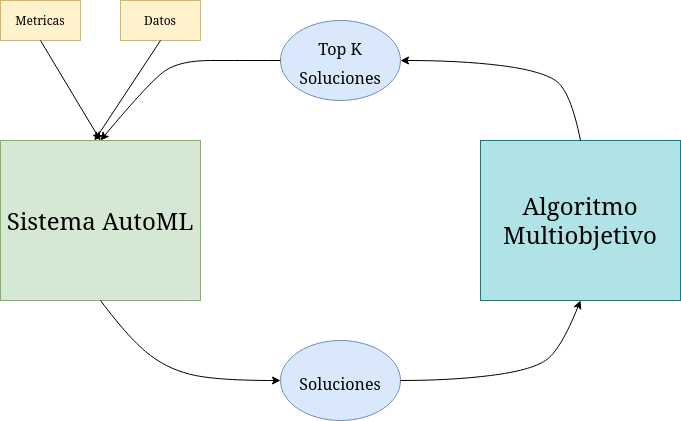
\includegraphics[scale=0.5]{Pictures/automl_moo_proposal.png}
    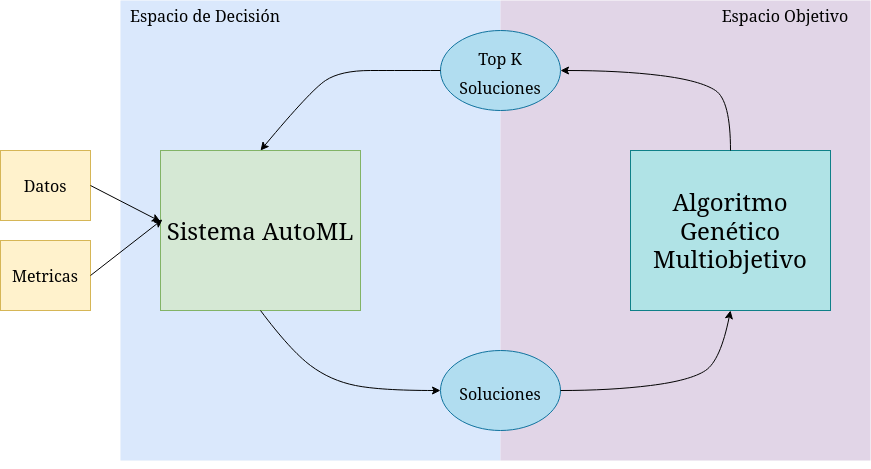
\includegraphics[scale=0.4]{Pictures/automl_moo_proposal2.png}
    \caption{Flujo general de la propuesta}
    \label{proposal:fig:flux}
\end{figure}

La soluci\'on propuesta (ver \ref{proposal:fig:flux}) est\'a compuesta por dos elementos fundamentales:
\begin{enumerate}
    \item Un sistema AutoML capaz de generar y evaluar m\'ultiples soluciones basado en un corpus de datos y un conjunto de m\'etricas. Generar nuevas soluciones partiendo de las soluciones m\'as aptas de la generaci\'on anterior.
    \item Un algoritmo de ordenaci\'on multiobjetivo capaz de funcionar solamente con el espacio objetivo y obtenga soluciones igualmente distribuidas a lo largo del frente de Pareto.
\end{enumerate}

La propuesta en cada iteraci\'on utiliza la evaluaci\'on de las soluciones generadas por el sistema de AutoML. La evaluaci\'on de una soluci\'on se representa como un vector $v$ de $m$ componentes donde $v_i$ es la evaluaci\'on de la soluci\'on con respecto a la m\'etrica $i$. El algoritmo ordena estos vectores utilizando alg\'un MOEA y retorna una lista ordenada de estos. Este proceso se repite hasta que se cumpla alg\'un criterio de parada.

La separaci\'on  por espacios existente entre ambas componentes de la propuesta permite que sean intercambiables. Todo sistema de AutoML que cumpla con estas condiciones es apto para la propuesta, no importa si est\'a enfocado en resolver el problema NAS o el problema CASH y toda algoritmo multiobjetvo capaz de producir ordenaciones efectivas utilizando solamente el espacio objetivo puede ser utilizado.
%generalizar el problema a cualquier tipo de sistema AutoML o funci\'on de ordenaci\'on.

% En su primera iteraci\'on el sistema AutoML debe producir una serie de soluciones y sus evaluaciones respectivas frente a las criterios de entrada. El algoritmo multiobjetivo debe ser capaz de ordenar efectivamente las soluciones de acuerdo a su evaluaci\'on tal que que los primeros $k$ elementos sean los m\'as aptos de para resolver el problema. Estas soluciones de mejor rendimiento se utilizan como entrada al sistema AutoML para que produzca una nueva generaci\'on de soluciones tomando la soluciones de entrada como referencia. El proceso se repite hasta que se cumpla el criterio de parada en donde se retornan los mejores individuos encontrados hasta el momento.

\subsection{Descripci\'on Formal}
El sistema propuesto est\'a compuesto por un sistema de Aprendizaje de M\'aquina Automatizado $\mathcal{A}(D, M, P)$  y un algoritmo evolutivo multiobjetivo $\mathcal{H}(TP)$. Los par\'ametros de entrada $D = \{(x_1, y_1), ..., (x_n, y_n)\}$ representa el conjunto de datos de entrada, $M = \{f_1, f_2, ..., f_m\}$ un conjunto de m\'etricas a evaluar, $P = \{p_1, p_2, ..., p_k\}$ el conjunto de soluciones de mejor rendimiento producidas por  $\mathcal{A}$ en la iteraci\'on anterior. $\mathcal{H}$ toma como entrada $TP$ que representa el conjunto de soluciones producidas en la iteraci\'on actual tras aplicar $\mathcal{A}(D, M, P)$. 
 %El objetivo final del sistema es producir una conjunto de soluciones de Aprendizaje Autom\'atico $P'$ que sean una muestra representativa del frente de Pareto (\ref{background:def:pareto_front}) utilizando un algoritmo multiobjetivo  $\mathcal{H}$ tal que $\mathcal{H}(TP) = P'$ en cierto n\'umero de iteraciones determinado por un criterio de parada. 
\begin{algorithm}[ht]\caption{Soluci\'on a AutoML Heter\'ogeneo Multiobjetivo}
    \KwIn{$\mathcal{A}$, D, M}
    \KwOut{P}
    $TP \gets \mathcal{A}(D, M, \emptyset)$ \tcp*{Se obtiene poblaci\'on inicial aleatoria}
    \While{no se cumplan condiciones de parada}{
        $P = \mathcal{H}(TP)$ \tcp*{Se extraen los m\'as aptos de una poblaci\'on} 
        $TP = \mathcal{A}(D, M, P)$ \tcp*{Se genera una nueva poblaci\'on}
    }
\end{algorithm}

% Tambi\'en debe ser capaz de entender las carectr\'isticas que componen las soluciones m\'as aptas tal que en las subsecuentes iteraciones estas se conserven. Lograr esto \'ultimo requiere que el sistema tenga en cierta medida una implementaci\'on de algoritmos gen\'eticos para construir sus soluciones, por ende, la propuesta se adapta mejor a sistemas AutoML que utilizen programaci\'on evolutiva.

\section{MOEA}
%El algoritmo trabaja con vectores debido a que optimiza para varias m\'etricas, y no con un escalar que es trivial organizar. Como se meciona en \ref{background:def:moo} se hablar ahora de dominaci\'on y el adecuado ordenamiento es vital para escoger puntos del espacio que: (i) pertenzcan a los mejores frentes, (ii) que sean los elementos representativos del frente

Esencialmente cualquier tipo de MOEA que sea suficiente informaci\'on sobre espacio objetivo se puede utilizar. Especif\'icamente para esta propuesta utilizamos una adaptaci\'on de NSGA-II (\cite{deb2002fast}) por ser un algoritmo que sigue una idea intuitiva y tiene un buen rendimiento general, suficiente para demostrar la efectividad de la propuesta.

\subsection{NSGA-II}
NSGA-II (\cite{deb2002fast}) es un algoritmo multiobjetvo basados en el frente de Pareto caracter\'isticos por dividir el proceso de selecci\'on de los individuos m\'as aptos en dos etapas:
\begin{itemize}
    \item \textit{Non Dominated Sorting} donde divide a la poblaci\'on basado en sus diferentes niveles de dominaci\'on.
    \item \textit{Crowding Distance Sorting} donde se dedicada a preservar la diversidad entre los individuos encontrados. 
\end{itemize}


\subsubsection{Non Dominated Sorting}
Durante esta etapa se agrupan las soluciones de acuerdo a su \'indice o nivel de dominaci\'on. Dicho \'indice est\'a  determinado por la cantidad de soluciones diferentes que la dominan.

\begin{definition}
    \label{proposal:def:domination_index}
    Dado un vector $x$ y un conjunto $Y$ de vectores en el espacio objetivo $\mathcal{Y}$ tal que los vectores en $Y$ dominan a $x$ (i.e. $Y = \{y | y \succ x\}$) se dice que $Ind(x) = |Y|$.
\end{definition}

\begin{definition}
    \label{proposal:def:rank_front}
    El conjunto de todas la soluciones con un mismo \'indice de dominaci\'on $i$ se les dice frente de rango $i$:
    \begin{equation*}
         F^i = \{x | x \in \mathcal{Y}, Ind(x) = i\}
    \end{equation*}
\end{definition}

El primer paso de \textit{Non Dominated Sorting} es calcular el \'indice de dominaci\'on de todas las soluciones revisando todos los pares de vectores $x, y \in \mathcal{Y}$ a la vez que se crea un grafo dirigido entre estos tal que existe una arista entre las soluciones $x$ y $y$ si $x \prec y$. Luego partiendo de las soluciones con nivel de dominaci\'on 0, visita todas las soluciones que estas dominan y les reduce el \'indice en uno. El proceso se repite hasta que no queden soluciones por analizar.
El resultado de esta primera etapa es una lista ordenada  $F = \{F^0, ..., F^k\}$ de todos los frentes de distinto rango obtenidos. 

%$F^0$ contiene las mejores vectores a los cuales nadie domina e idealmente ser\'ia una aproximaci\'on al frente de Pareto.

%Es importante entender para la correctitud del aloritmo anterior  que las soluciones que conforman un frente de rango $i$ no se \textit{Pareto dominan} ($\prec$) entre si.
%Es f\'acilmente demostrable que la \texit{Pareto dominacion (i.e. $\prec$)} cumple con la propiedad de transitividad (i.e. si $x \prec y$, $y \prec z$, entonces $x \prec z$) 
%\begin{theorem}
%Dado $P^i$, frente de rango $i$, resultado de efectuar obtenido por Non Dominated Sort sobre una conjunto soluci\'on entonces $\neg \exists x, y \in P^i$ tal que $x \prec y$
%\end{theorem}
%% Definir correctamente la prueba
%Dado un frente de rango $i$ $F_i$, tal que existen soluciones $x, y \in F_i$ se asume que $x \prec y$. Como el \'inidice de dominaci\'on de $x$ es $i$ y $x \prec y$ y ($\prec$) es una operador transitivo entonces todos los que dominan a $x$ dominan a $y$, adem\'as del propio $x$, por tanto el inidice de dominaci\'on de $y$ ser\'ia $i+1$ lo que es una contradicci\'on porque $y \in F_i$. 

\subsubsection{Crowding Distance Sorting}
\textit{Crowding Distance Sorting}(CD), uno de los aportes claves hechos por NSGA-II, se utiliza sobre  $F^i$ un frente de rango $i$ obtenido en la etapa anterior con el objetivo de ordenar sus elementos seg\'un cuan representativos del conjunto sean. Esta parte es vital pues permite que en los casos donde haya que utilizar solo la porci\'on de un frente, se utilize la m\'as representativa de este manteniendo la diversidad del conjunto.
%En la segunda etapa los vectores de cada frente obtenido se organizan utilizando \textit{crowding distance} (CD), uno de las contribuciones claves de NSGA-II (\cite{deb2002fast}). El prop\'osito de \textit{crowding distance} es estimar la densidad de las soluciones con respecto sus soluciones vecinas de tal manera que los primeros lugares pertenezcan a los elementos m\'as representativos de dicho frente.

% Imagen de crowding distance
Calcular el CD de cada soluci\'on require ordenarlas seg\'un su valor normalizado por cada funci\'on objetivo y calcular el promedio de la distancia entre una soluci\'on y sus dos adyacentes respecto a dicha funci\'on objetivo. Esta distancia es el per\'imetro del cuboide formado utilizando los vecinos m\'as cercanos como v\'ertices. Los puntos que representan el m\'inimo y m\'aximo de al menos alguna funci\'on objetivo se les asigna \textit{crowiding distance} infinita. El  algoritmo queda descrito en \ref{proposal:alg:cd}.

\begin{algorithm*}[ht]
    \caption{Crowding Distance Sorting}
    \label{proposal:alg:cd}

    \tcp{F como entrada representa un frente de rango i}
    \KwIn{F} 
    \tcp{SF como salida representa el frente ordenado seg\'un CD}
    \KwOut{SF}
    \For{i desde 0 hasta $|F|$}{
        $F[i].dist \gets 0$ \;
    } 

    \ForEach{funcion objetivo $m$}{
        $F \gets ordenar(F, m)$ \tcp*{se ordena F con respecto a m}
        $F[0].dist \gets \infty$\;
        $F[|F|].dist \gets \infty$\;

        \For{i desde 2 hasta $|F| - 1$} {
            \begin{math}
                F[i].distance  = F[i].distance + \frac{(F[i + 1].m - F[i - 1].m)}{f^{max}_{m} - f^{min}_m}
            \end{math}
        }
    }
    $SF \gets ordenar(F, dist)$ \tcp*{se ordena F respecto a CD}
\end{algorithm*}

\subsubsection{Ciclo Prinicipal}
Inicialmente se crea una poblaci\'on aleatoria $P_0$ de soluciones de tama\~no $N$. Cada soluci\'on es ordenada de acuerdo a \textit{Non Dominated Sorting} y se aplica un torneo binario utilizando operadores gen\'eticos de selecci\'on, recombinaci\'on y mutaci\'on para crear una poblaci\'on decendiente $Q_0$ de tama\~no $N$.

Luego se forma una poblaci\'on $R_t = P_t \cup Q_t$ de tama\~no 2N. La poblaci\'on $R_t$ es ordenada de acuerdo al nivel de dominaci\'on de cada individuo obteni\'endose una lista de frentes de distinto rango $F = \{F^0, ..., F^k\}$. Las soluciones en $F^0$ representan las mejores soluciones encontradas por el algoritmo hasta el momento y es necesario que pasen a formar parte de la poblaci\'on de la siguiente iteraci\'on $P_{t+1}$. Si $|F^0| < N$ el frente completo pasa formar parte de $P_{t+1}$. Los miembros restantes de la nueva poblacion son escogidos de los dem\'as frentes acorde a su \'indice de dominaci\'on. Si $F^k$ no capaz de pertencer completo a $P_{t+1}$ debido a que $\sum_0^k |F^i| > N$ se aplica \textit{Crowding Distance Sorting} sobre $F^k$ y se llena las posiciones restantes con los individuos de mayor distancia.

La nueva poblaci\'on $P_{t+1}$ se utiliza para producir una poblci\'on $Q_{t+1}$ con operadores de selecci\'on, cruzamiento y mutaci\'on. El procedimiento general de NSGA-II se muestra en la figura \ref{proposal:fig:nsga2}.

\begin{figure}[ht]
    \centering
    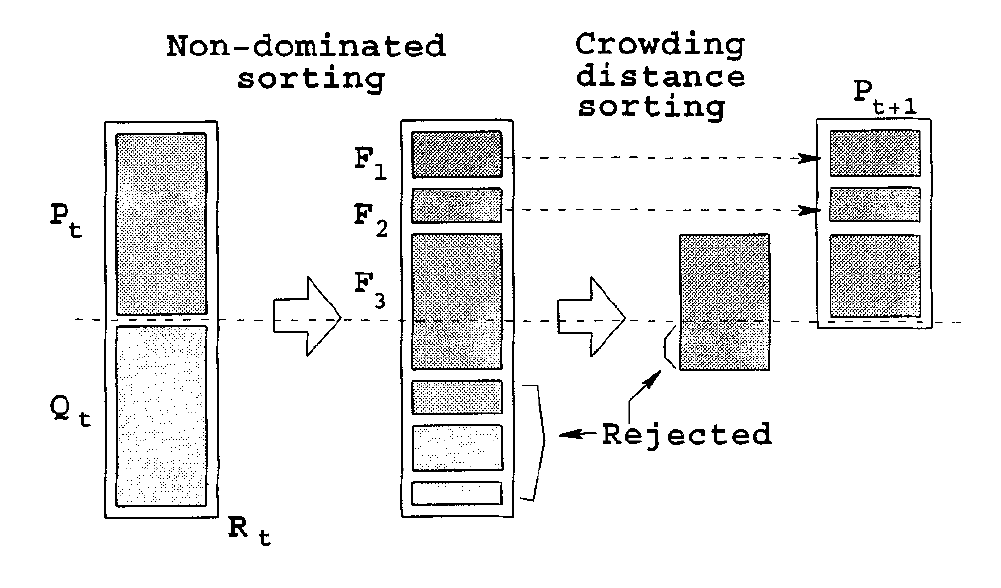
\includegraphics[scale=0.5]{Pictures/nsga2.png}
    \caption{Funcionamineto de NSGA-II}
    \label{proposal:fig:nsga2}
\end{figure}

\subsection{NSGA-II Generalizado}

NSGA-II realiza una serie de asunciones sobre las poblaciones con las que trabajan que no lo hacen perfectamente integrable con nuestra propuesta. Proponemos una adaptaci\'on del algoritmo que conserva sus dos etapas de ranking fundamentales pero con un ciclo principal m\'as sencillo que no aplica operadores gen\'eticos ni modificaciones sobre la poblaci\'on limit\'andolo al espacio objetivo $\mathcal{Y}$.

\subsubsection{Ciclo Prinicipal}
El ciclo de nuestra propuesta recibe una poblaci\'on inicial $P$ de tama\~no N y pasa directamente a aplicar \textit{Non Dominated Sorting} con los que se obtiene una lista de frentes de distinto rango $F = \{F^0, ..., F^l\}$ con el objetivo de formar un conjunto $P'$ de tama\~no $k$ que representen los mejores elementos de $P$. Las soluciones que pasan a formar parte de $P'$ se escojen a\~nadiendo en grupos por cada frente $F^i$ hasta que cierto frente $F^q$ que no pueda a\~nadirse completo. Los puestos restantes se llenan con los elementos de mayor distanica de $F^q$ tras aplicar \textit{Crowding Distance}.

Se simplifica el ciclo respetando la idea de la propuesta general.  Los sistemas AutoML son los que deciden como generar soluciones y que hacer con la informaci\'on de los m\'as aptos, permitiendo que se puedan utilizar como una caja negra intercambiable.

% Picar el capitulo entre Implementacion y Experimentos
% Añadir un p\'arrafo al final de Implementacion de como se utilza el nuevo sistema
\chapter{AutoGOAL Multiobjetivo}\label{chapter:implementation}
En este cap\'itulo se muestra una implmentaci\'on la propuesta utilizando a AutoGOAL (\cite{estevez2020solving}) como sistema de AutoML. AutoGOAL modela el espacio de b\'usqueda utilizando algoritmos evolutivos y nuestra propuesta consiste en seleccionar las mejores respuestas dada su evaluaci\'on.  AutoGOAL modela el espacio de b\'usqueda utilizando algoritmos evolutivos. Antes de explicar la implementaci\'on es necesario entender la base te\'orica sobre la que se apoya AutoGOAL para modelar el espacio  de b\'usqueda. 

\section{Marco Te\'orico de AutoGOAL}

AutoGOAL (\cite{estevez2020solving}) modela su espacio de decisi\'on basado una Gram\'atica Probabil\'istica  Libre del Contexto (\textit{Probabilistic Context Free Grammar}, PCFG) y utiliza Evoluci\'on Gram\'atica Probabil\'istica (\textit{Probabilistic Grammatic Evolution} para dirigir la b\'usqueda dentro de este espacio. 

PCFG se define como una quinterna $PCFG = (NT, T, S, P, Prob)$ donde $NT$ y $T$ representan los conjuntos disjuntos no vac\'io de los s\'imbolos no terminales y terminales respectivamente. $S$ representa el No Terminal inicial con el que es posible expandir toda la gram\'atia. $P$ es el conjunto de reglas de producci\'on que rigen a la grma\'atica. $Prob$ (el elemento que hace que sea diferente que las gram\'aticas libres de contexto en general) es un conjunto de probabilidades asocaido con cada producci\'on de la gram\'atica. 

Para acutalizar el espacio de decisi\'on  se utiliza Evoluci\'on Gram\'atica Probabil\'istica (\textit{Probabilistic Grammatic Evolution}, PGE, \cite{megane2021probabilistic}), un algorimto de Estimaci\'on de Distribuci\'on (\textit{Estimation of Distribution ALgorithms, EDA}, \cite{larranaga2001estimation}) que remplaza los operadores cl\'asicos de mutaci\'on y cruce por un muestreado sobre las probabilidades de distribuci\'on de PCFG de acuerdo a las producciones utilizadas por el mejor individuo. 

\section{Implementaci\'on}

\begin{figure}[ht]
    \centering
    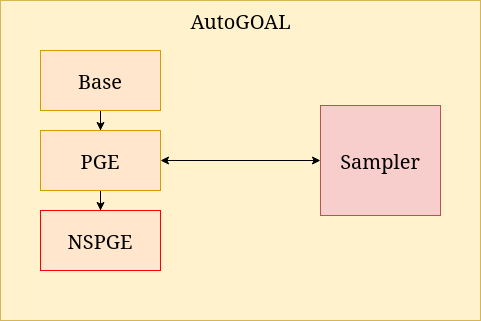
\includegraphics[scale=0.6]{Pictures/autogoal_impl.png}
    \caption{Diagrama general}
    \label{impl:fig:general_diagram}
\end{figure}


AutoGOAL es un sistema de AutoML gen\'etico que utiliza una Gram\'atica Probabil\'istica Libre del Contexto  para modelar su espacio de decisi\'on. Se representa utilizando un grafo aciclico dirigido (DAG) donde cada nodo de este representa una posible cadena de la gram\'atica y sus aristas apuntan a todas las posibles cadenas que se pueden generar a partir de estas sustituyendo alg\'un No Terminal por una producci\'on de la Gram\'atica. Cuando una cadena se encuentra completamente expandida, i.e. compuesta por solo simbolos terminales, se tiene una soluci\'on v\'alida del sistema. 

Inicialmente cada arista de este DAG se inicializa con una probabilidad igual a todas sus aristas hermanas (i.e. todas las aristas que salen de su mismo nodo) tal que la suma de sus probabilidades sea 1. Un camino se escoge utilizando una variable uniforme tal que su valor determina la arista a seleccionar. Cuando se tiene un individuo apto la manera de AutoGOAL de conservar sus ``genes'' es aplicando PGE sobre las aristas que conforman el camino que llevaron a esa soluci\'on. M\'as especificamente, la implementaci\'on de AutoGOAL de PGE dado $n$ individuos, son evaluados respecto a una funci\'on de evaluaci\'on $f$ y se crea una listas de las $k$ mejores soluciones (encabezada por la m\'as apta) y las aristas de las probabilidades se actualizan de acuerdo a estas soluciones. 

Se a\~nade a AutoGOAL la clase NSPGE, un m\'etodo de b\'usqueda inspirado en NSGA-II (\cite{deb2002fast}) que utiliza PGE como base. El objetivo de NSPGE es extender la funcionalidad de PGE para que sea capaz de seleccionar los $k$ mejores individuos de acuerdo a $m$ m\'etricas, con $m \ge 2$. La l\'ogica de la PGE encargada de ordenar los inidividuos m\'as aptos se encuentra en el m\'etodo \textit{\_inidices\_of\_the\_fittest\_} la cual NPSGE sobreescribe.

\subsection{NSPGE}

En NSPGE, dentro de \textit{\_inidices\_of\_the\_fittest\_} se aplica la ordenaci\'on definida por \cite{deb2002fast}. Dado $n$ soluciones se  agrupan seg\'un su \'indice de dominaci\'on (i.e. Non Dominated Sorting), donde cada agrupamiento se le llama frente de rango $i$, donde $i$ representa la cantidad de soluciones que dominan a cada una de estas. Una vez establecidos estos frentes se extraen las primeras $k$ soluciones, en caso de que no se pueda seleccionar un frente completo, se aplica Crowding Distance para seleccionar la muestra m\'as representativa de este.


\begin{lstlisting}[caption=Nueva ordenaci\'on, language=Python]
def _indices_of_fittest(self, fns: List[List[float]]):
  # Se ordenan todas las soluciones segun su orden
  # de dominacion
  fronts = self.non_dominated_sort(fns)
  indices = []
  k = int(self._selection * len(fns))

  for front in fronts:
    if len(indices) + len(front) <= k:
      indices.extend(front)
    else:
      # Cuando solo se utiliza una porcion del frente
      # se aplica crowding distance
      indices.extend(
          sorted(
              front,
              key=lambda i: -self.crowding_distance(fns, front, i)
          )[: k - len(indices)]
      )
      break
  return indices
\end{lstlisting}

\subsubsection{Non Dominated Sort}
La ordenaci\'on se conforma por dos pasos l\'ogicos fundamentales:
\begin{enumerate}
    \item Se verifica todo par de soluciones $x, y$ encontradas y se aplica $x \prec y$ con el objetivo de calcular el \'inidice de dominaci\'on de cada soluci\'on. Adem\'as se construye un DAG conformado por las soluciones donde existe una arista entre las soluciones $x$ y $y$ si $x \prec y$. La ra\'iz de dicho DAG est\'a conformado por las soluciones que nadie domina.
    \item Se recorre DAG utilizando una versi\'on de BFS ($Breadth First Search$) donde los soluciones visitadas se les reduce el \'indice de domianci\'on en uno. Si llega a 0 se a\~nade al frente de Pareto que se est\'a formando.
\end{enumerate}

\begin{lstlisting}[caption=Non Dominated Sorting, language=Python]
def non_dominated_sort(self, scores: List[List[float]]):
  # fronts almacena los frentes 
  #(i.e. fronts[i] es el frente de rango i)
  fronts: List[List[int]] = [[]]

  # domination_rank en i indica la cantidad de soluciones
  # que dominan a la solucion i
  domination_rank = [0] * len(scores)

  # dominated_scores en i alamacena las soluciones dominadas
  # por la solucion i
  dominated_scores = [list() for _ in scores]

  # revisa todo par de soluciones y se establece
  # quien dominan a quien
  for i, score_i in enumerate(scores):
    for j, score_j in enumerate(scores):
      if self._improves(score_i, score_j):
          dominated_scores[i].append(j)
      elif self._improves(score_j, score_i):
          domination_rank[i] += 1
    if domination_rank[i] == 0:
       fronts[0].append(i)

  # de acuerdo a la informacion sobre quienes
  # se dominan, forma todos los frentes
  front_rank = 0
  while len(fronts[front_rank]) > 0:
    next_front = []
    for i in fronts[front_rank]:
      for dominated in dominated_scores[i]:
        domination_rank[dominated] -= 1
        if domination_rank[dominated] == 0:
          next_front.append(dominated)
    front_rank += 1
    fronts.append(next_front)

  return fronts[:-1]
\end{lstlisting}

\subsubsection{Crowding Distance}
Se sigue la idea del algoritmo propuesto en (\ref{proposal:alg:cd}). Dado $m$ m\'etricas a evaluar se realizan $m$ iteraciones, donde en cada una se ordena alg\'un frente de rango $k$ de acuerdo a la metrica $m_i$. A la soluciones que con respecto a la m\'etrica $m_i$ tienen el m\'inimo y mayor valor se les asigna distancia infinita y luego se c\'alculan los valores intermedios. En \cite{deb2002fast} requiren que los valores de las m\'etricas esten normalizados, en nuestra implementaci\'on utilizamos \textit{feature scaling} para normalizar los valores entre 0 y 1.

\begin{lstlisting}[caption=Crowding Distance Sorting, language=Python]
def crowding_distance(
    self, scores: List[List[float]], front: List[int], index: int
) -> float:
  # Crowding distance usa los vectores normalizados.
  # Se aplica feature scaling para llevar los vectores a [0, 1]
  scaled_scores = feature_scaling(scores)

  crowding_distances: List[float] = [0 for _ in scores]
  for m in range(len(self._maximize)):
    # Se ordena de acuerdo a la metrica m
    front = sorted(front, key=lambda x: scores[x][m])

    # Se establecen los extremos como infinitos
    crowding_distances[front[0]] = math.inf
    crowding_distances[front[-1]] = math.inf

    # Valores de todas las soluciones con respecto a m 
    m_values = [scaled_scores[i][m] for i in front]
    scale: float = max(m_values) - min(m_values)
    if scale == 0:
      scale = 1
    for i in range(1, len(front) - 1):
      crowding_distances[i] += (
        scaled_scores[front[i + 1]][m] - scaled_scores[front[i - 1]][m]
      ) / scale

  return crowding_distances[index]
\end{lstlisting}

\section{Utilizar la Implementaci\'on}

La soluci\'on representa la adici\'on de un nuevo m\'etodo de b\'usqueda. Para utilizarla es necesaria especificarla como un par\'ametro de la b\'usqueda.

Para especificar las m\'etricas multiobjetivo la funci\'on de puntuaci\'on se define el retorno como una tupla de elementos.

Adem\'as se le pasa al algoritmo una tupla de tama\~no similar a la cantidad de metricas que indique por cada posicion $i$ si la m\'etrica $i$ es de minimizar o maximizar

\begin{lstlisting}[caption=Utilizando NPSGE, language=Python]
from autogoal.datasets import cars
from autogoal.kb import MatrixContinuousDense, Supervised, VectorCategorical
from autogoal.ml import AutoML
from autogoal.utils import Gb, Hour, Min
from autogoal.search import NSPESearch
from utils import plot_and_save, print_and_save

automl = AutoML(
    input=(MatrixContinuousDense, Supervised[VectorCategorical]),
    output=VectorCategorical,
    pop_size=40,
    score_metric=accuracy_vs_time,
    search_algorithm=NSPESearch,
    maximize=(True, True),
    random_state=2,
    number_of_solutions=100,
    memory_limit=16 * Gb,
    search_timeout=1 * Hour,
)

x, y = cars.load()
automl.fit(x, y)


\end{lstlisting}

\chapter{Experimentaci\'on y Resultados}\label{chapter:experiments}
En este cap\'itulo se eval\'uan los resultados obtenidos por AutoGOAL Multiobjetivo tras aplicarse sobre tres corpus de datos utilizando los pares de m\'etricas precis\'on contra recobrado y \textit{f-score} contra tiempo de entrenamiento:
\begin{itemize}
    \item Precisi\'on es una m\'etrica que mide las muestras clasificadas correctamente entre todas las muestras extra\'idas.
    \item Recobrado mide las muestras clasificadas correctamente sobre todas las extra\'idas.
    \item \textit{F-score} es el promedio arm\'onico entre precisi\'on y recobrado.
    \item \textit{Tiempo de entrenamiento} es un estimado que mide cuanto tiempo toma para una flujo de Aprendizaje Autom\'atico en realizar el proceso de entrenamiento.
\end{itemize}

Se utiliza el par de metricas precisi\'on y recobrado pues son criterios que pueden tener comportamientos variados. Existen problemas donde es posible maximizar ambas y otros donde es obligatorio realizar concesiones entre estas tal que no exista una mejor soluci\'on sino un conjunto de estas.

Se utilza \textit{f-score} contra tiempo de entrenamiento para probar si es posible dirigir efectivamente  la b\'usqueda maximizando la relevancia y minimizando el tiempo de ejecuci\'on. Es posible utilzar tambi\'en precisi\'on y recobrado junto con tiempo de entrenamiento pero con el objetivo de mantener estos primeros experimentos m\'as sencillos se utiliza \textit{f-score}.

\section{Corpus de Evaluaci\'on}
Se utilizan tres corpus de datos para comprobar el comportamiento del sistema cuando optimiza para varias m\'etricas simult\'aneamente. Los corpus se escogen de distintos tamaños y cada uno representa versiones distintas del problema de aprendizaje supervisado.

\subsection{CARS}
Cars (\cite{Dua:2019}) es un corpus que representa un conjunto de carros con ciertas caracter\'isticas catalogadas cualitativamente (ver \ref{implementation:table:cars:attributes}). El objetivo con este corpus es aprender a clasificar los carros de  acuerdo a sus atributos  en inaceptable, aceptable, bueno o muy bueno (\ref{implementation:table:cars:classes}). El corpus no tiene valores desconocidos.

\begin{table}[ht]
    \centering
    \parbox{.45\linewidth}{
    \begin{tabular} { |l|c| }
        \hline
        Atributos & Valores \\
        \hline
        \hline
        buying & v-high, hihg, med, low \\
        \hline
        maintance &  v-high, hihg, med, low\\
        \hline
        doors & 2, 3, 4, 5-more\\
        \hline
        persons & 2, 4, more\\
        \hline
        lug\_boot & small, med, big\\
        \hline
        safety & low, med, high\\
        \hline
    \end{tabular}
    \caption{Tipos de Atributos en Cars}
    \label{implementation:table:cars:attributes}
    }
    \qquad
    \parbox[t]{.45\linewidth}{
    \begin{tabular} {|l|c|c|}
        \hline
        Clases & N & \% \\
        \hline
        \hline
        unacc & 1210 & 70.023\%\\
        \hline
        acc & 384 & 22.222\%\\
        \hline
        good & 69 & 3.993\%\\
        \hline
        v-good & 65 & 3.762\%\\
        \hline
    \end{tabular}
    \caption{Distribuci\'on de clases en Cars}
    \label{implementation:table:cars:classes}
    }
\end{table}

\subsection{HAHA}
Humor Analysis based on Human Annotation (\cite{chiruzzo2019overview}) representa un conjunto de datos que contiene \textit{tweets} en espa\~nol en texto plano codificado en utf-8. Se quiere construir un clasificador que pueda catalogarlos correctamente entre si son humor\'isticos o no. Contiene un total de 30000 tweets donde se utilizan 24000 para entrenamiento y 6000 para evaluaci\'on.

\begin{table}[ht]
    \centering
    \begin{tabular} {|l||c|c|c|}
        \hline
        & Entrenamiento & Evaluaci\'on & Total \\
        \hline
        \hline
        Tweets & 24000 & 6000 & $30000$\\
        \hline
        Graciosos & 9253 & 2342 & 11595\\
        \hline
        No graciosos & 14 757 & 3 658 & 18 405\\
        \hline
        Puntuaci\'on Promedio & 1305 & 275 & 1580\\
        \hline
    \end{tabular}
    \caption{Distribuci\'on de clases en HAHA}
    \label{implementation:table:haha}
\end{table}

\subsection{MEDDOCAN}

\textit{Spanish Clinical Case Corpus - Medical Document Anonymization} (MEDDOCAN, \cite{marimon2019automatic}) representa colecci\'on de 1000 casos cl\'inicos y sus anotaciones PHI. Cada uno est\'a conformado con aproximadamente de 33 oraciones o 495 palabras. Los caso cl\'inico est\'an codificados en texto plano en utf-8 y las anotaciones est\'an en formato BRAT. El objetivo es predecir dichas anotaciones.

\section{Hardware}
 Los experimentos fueron ejecutados en un equipo con las siguientes propiedades: CPU AMD R5 3550h y 32 GB de RAM.

\section{Resultados y An\'alisis}

En esta secci\'on se muestran los resultados obtenidos tras aplicar AutoGOAL Multiobjetivo a los distintos corpus. En las gr\'aficas solo se tiene en cuenta la puntuaci\'on de relevancia obtenida durante entrenamiento y no con respecto a los datos de prueba. Los puntos  grises marcan las mejores soluciones encontradas en cada generaci\'on.  La tonalidad de los puntos var\'ia de acuerdo en que iteraci\'on del algoritmo fue encontrado; a medida que avanzan las generaciones estos se oscurecen. Los puntos marcados con cruces rojas representan las mejores soluciones encontradas por el algoritmo y conforman una aproximaci\'on del frente de Pareto.

En cada conjunto de datos se utilizaron param\'etros distintos debido fundamentalmene a que cada corpus representa problemas con diferente complejidad y cantidad de datos.

\subsection{Cars}
La aplicaci\'on de AutoGOAL en Cars utiliza una poblaci\'on total de 40 individuos por generaci\'on, 1 hora de tiempo m\'aximo y 10 segundos de tiempo l\'imite por \textit{pipeline}. Se utilizaron las implementaciones de \textit{f-score}, \textit{precision} y \textit{recall} de scikit-learn (\cite{pedregosa2011scikit}) con el promedio \textit{weighted} utilizado para problemas de clasificaci\'on multiclase que pueden tener un desbalance en las clases existentes.

\subsubsection{F-Score contra Tiempo de Entrenamiento}
La mayor\'ia de las soluciones encontradas componen un frente de Pareto con una forma extra\~na aparentemente c\'oncava pero bien distribuida sobre el espacio (ver figura \ref{impl:fig:cars:fscore_vs_time}).  El sistema encuentra  m\'ultiples soluciones de muy buen \textit{f-score} la mayor\'ia dirigidas a minimizar el tiempo de entrenamiento. 

L.os algoritmos que logran una puntuaci\'on de 1.0 tiene en com\'un que todos utilizan \textit{Suppport Vector Machines} (SVC). En el rango de 0.7 a 0.9 se encuentran pipelines con distintas t\'ecnicas como \textit{Nearest Centroid}, \textit{Multinomial Naive Bayes}, \textit{Bernoulli Naive Bayes} y SVC l\'ineal.

\begin{figure}[ht]
    \centering
    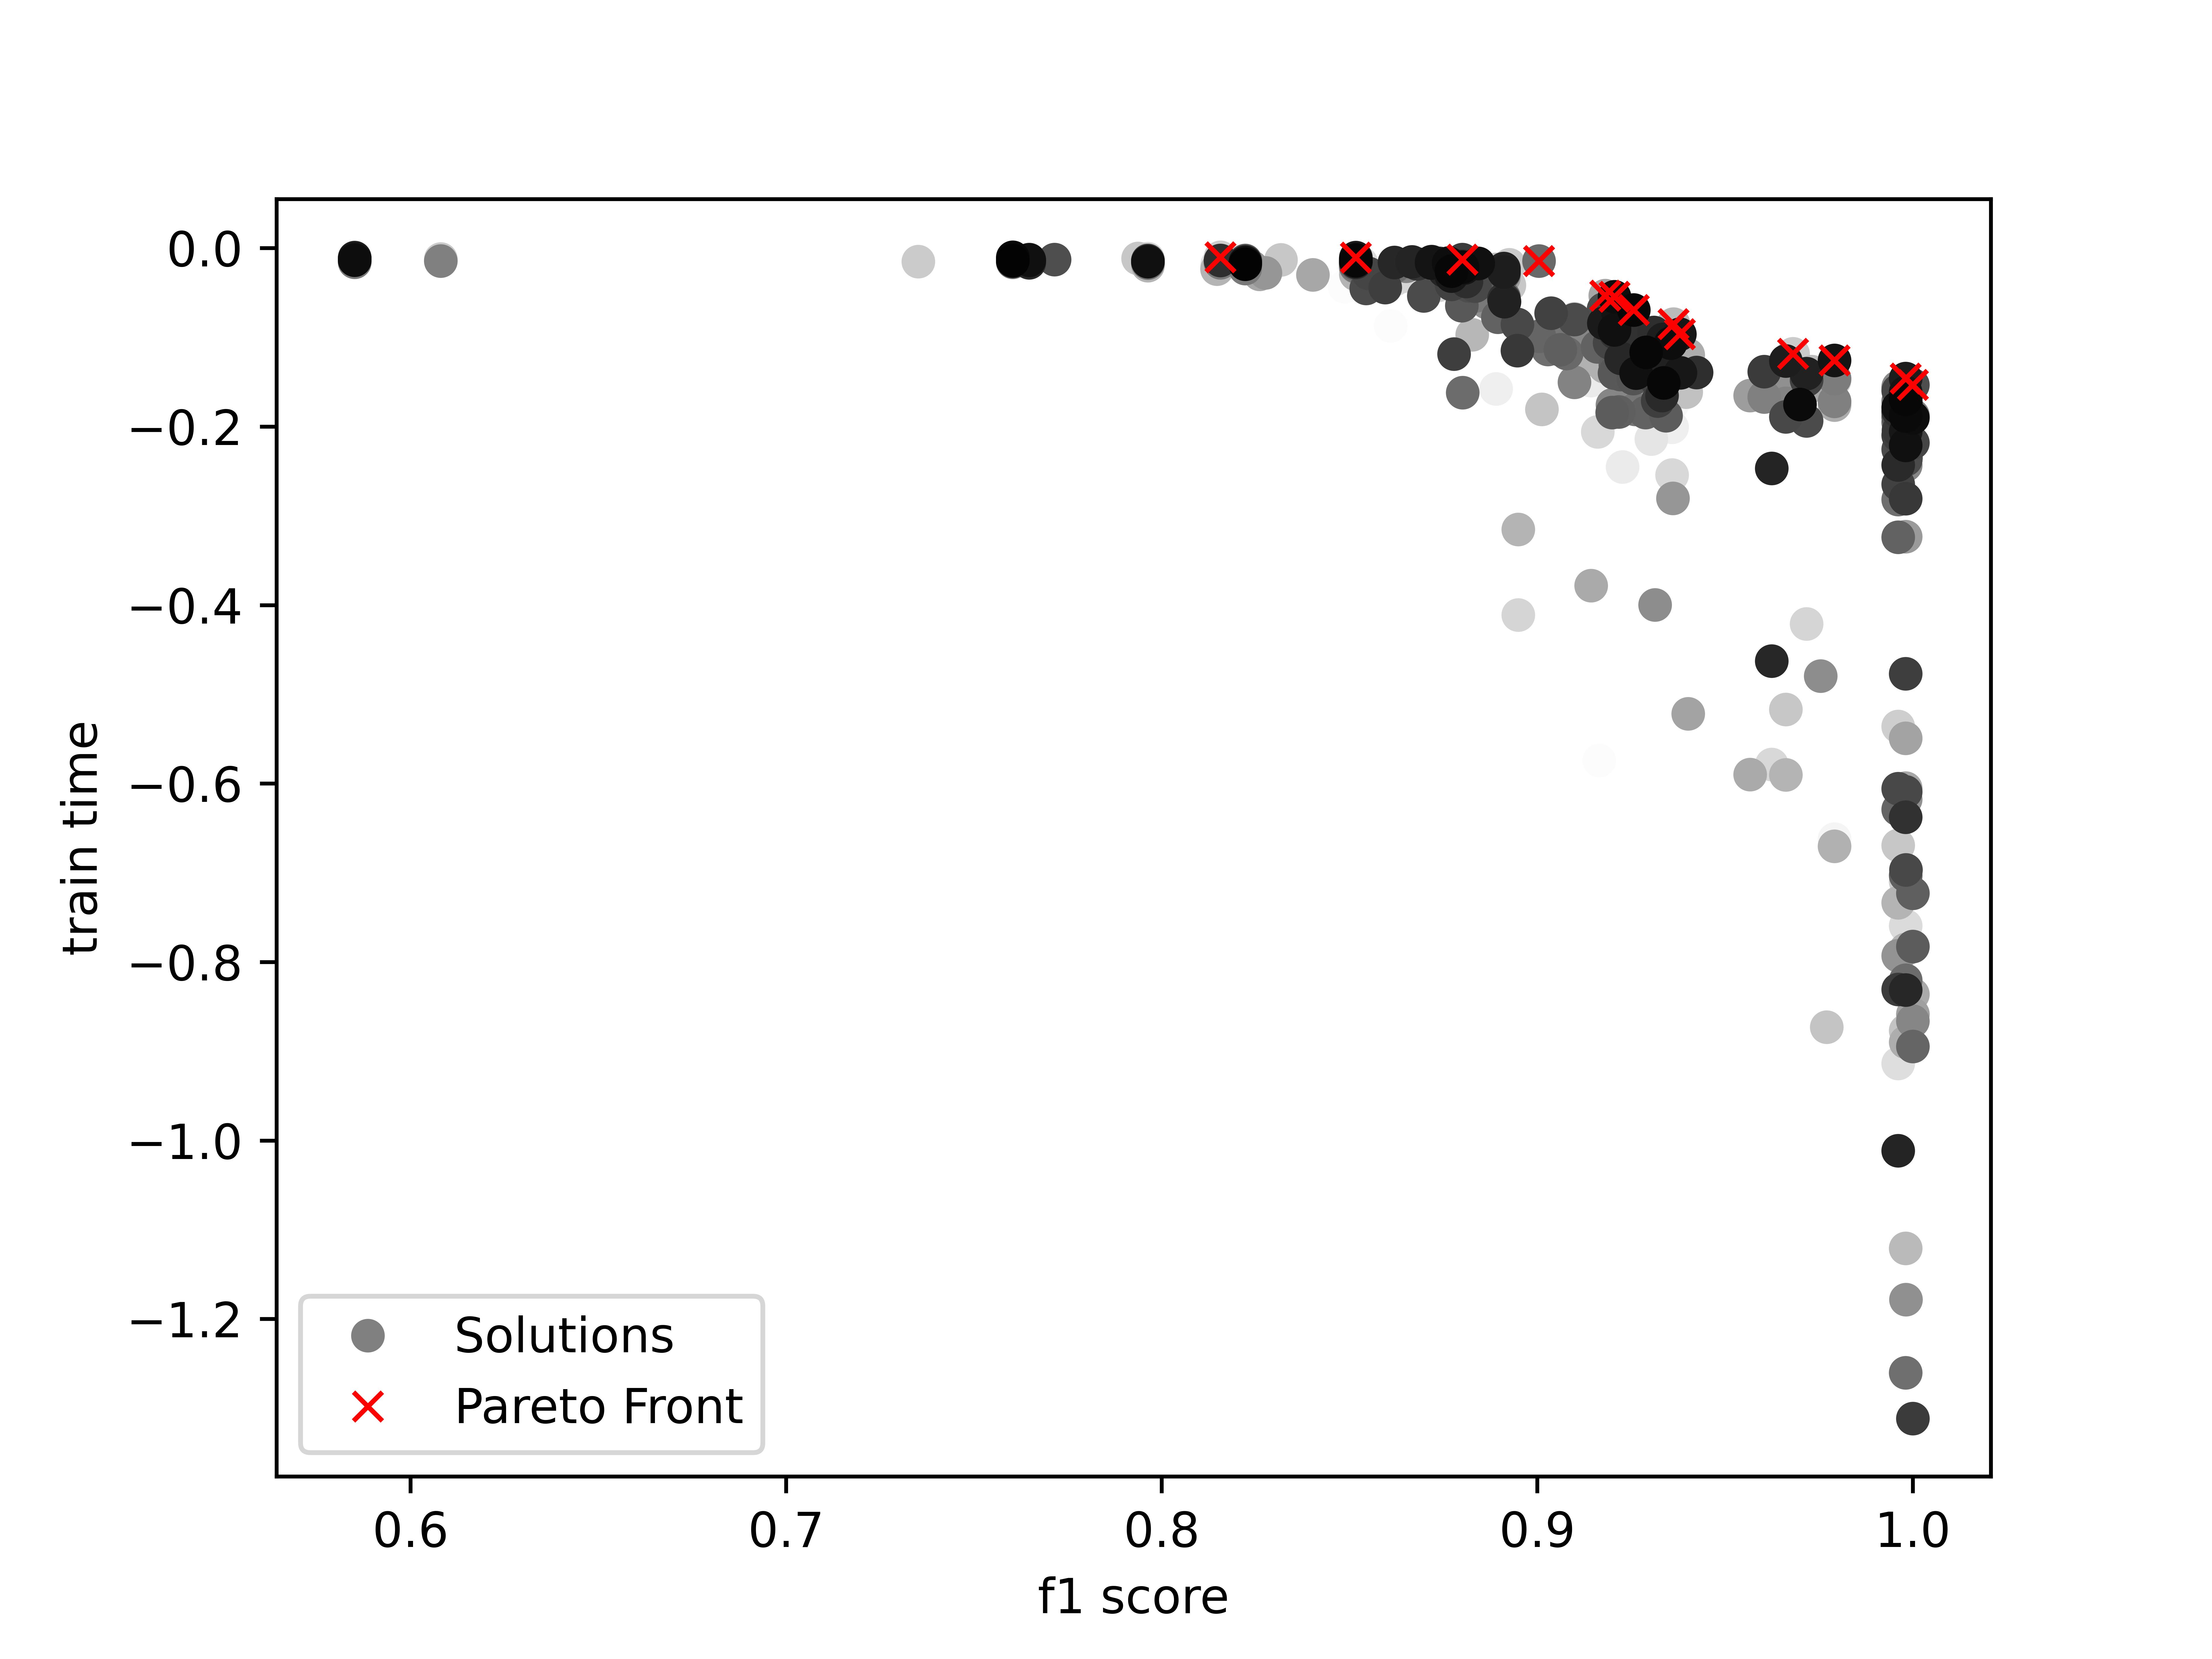
\includegraphics[scale=0.65]{Pictures/cars_fscore_vs_time.jpg}
    \caption{Cars: F-score contra Tiempo de Entrenamiento}
    \label{impl:fig:cars:fscore_vs_time}
\end{figure}


\subsubsection{Precisi\'on contra Recobrado}
Durante esta prueba  ni precisi\'on ni recobrado entr\'an en conflicto y por tanto no es necesario hacer concesiones entre una o la otra durante la optimizaci\'on. Se puede observar en la figura \ref{impl:fig:cars:precision_vs_recall} que el frente de Pareto esta consituido por un s\'olo punto donde se maximizan precisi\'on y recobrado. Tambi\'en se nota como las soluciones van mejorando con el transcurso de las iteraciones.

AutoGOAL encontr\'o 5 soluciones compuestas, entre otras t\'ecnicas, por SVC con un rendimiento perfecto. En este caso hay flujos m\'as complejos con respecto a la prueba anterior pues no se discrimina por tiempo de entrenamiento.

\begin{figure}[ht]
    \centering
    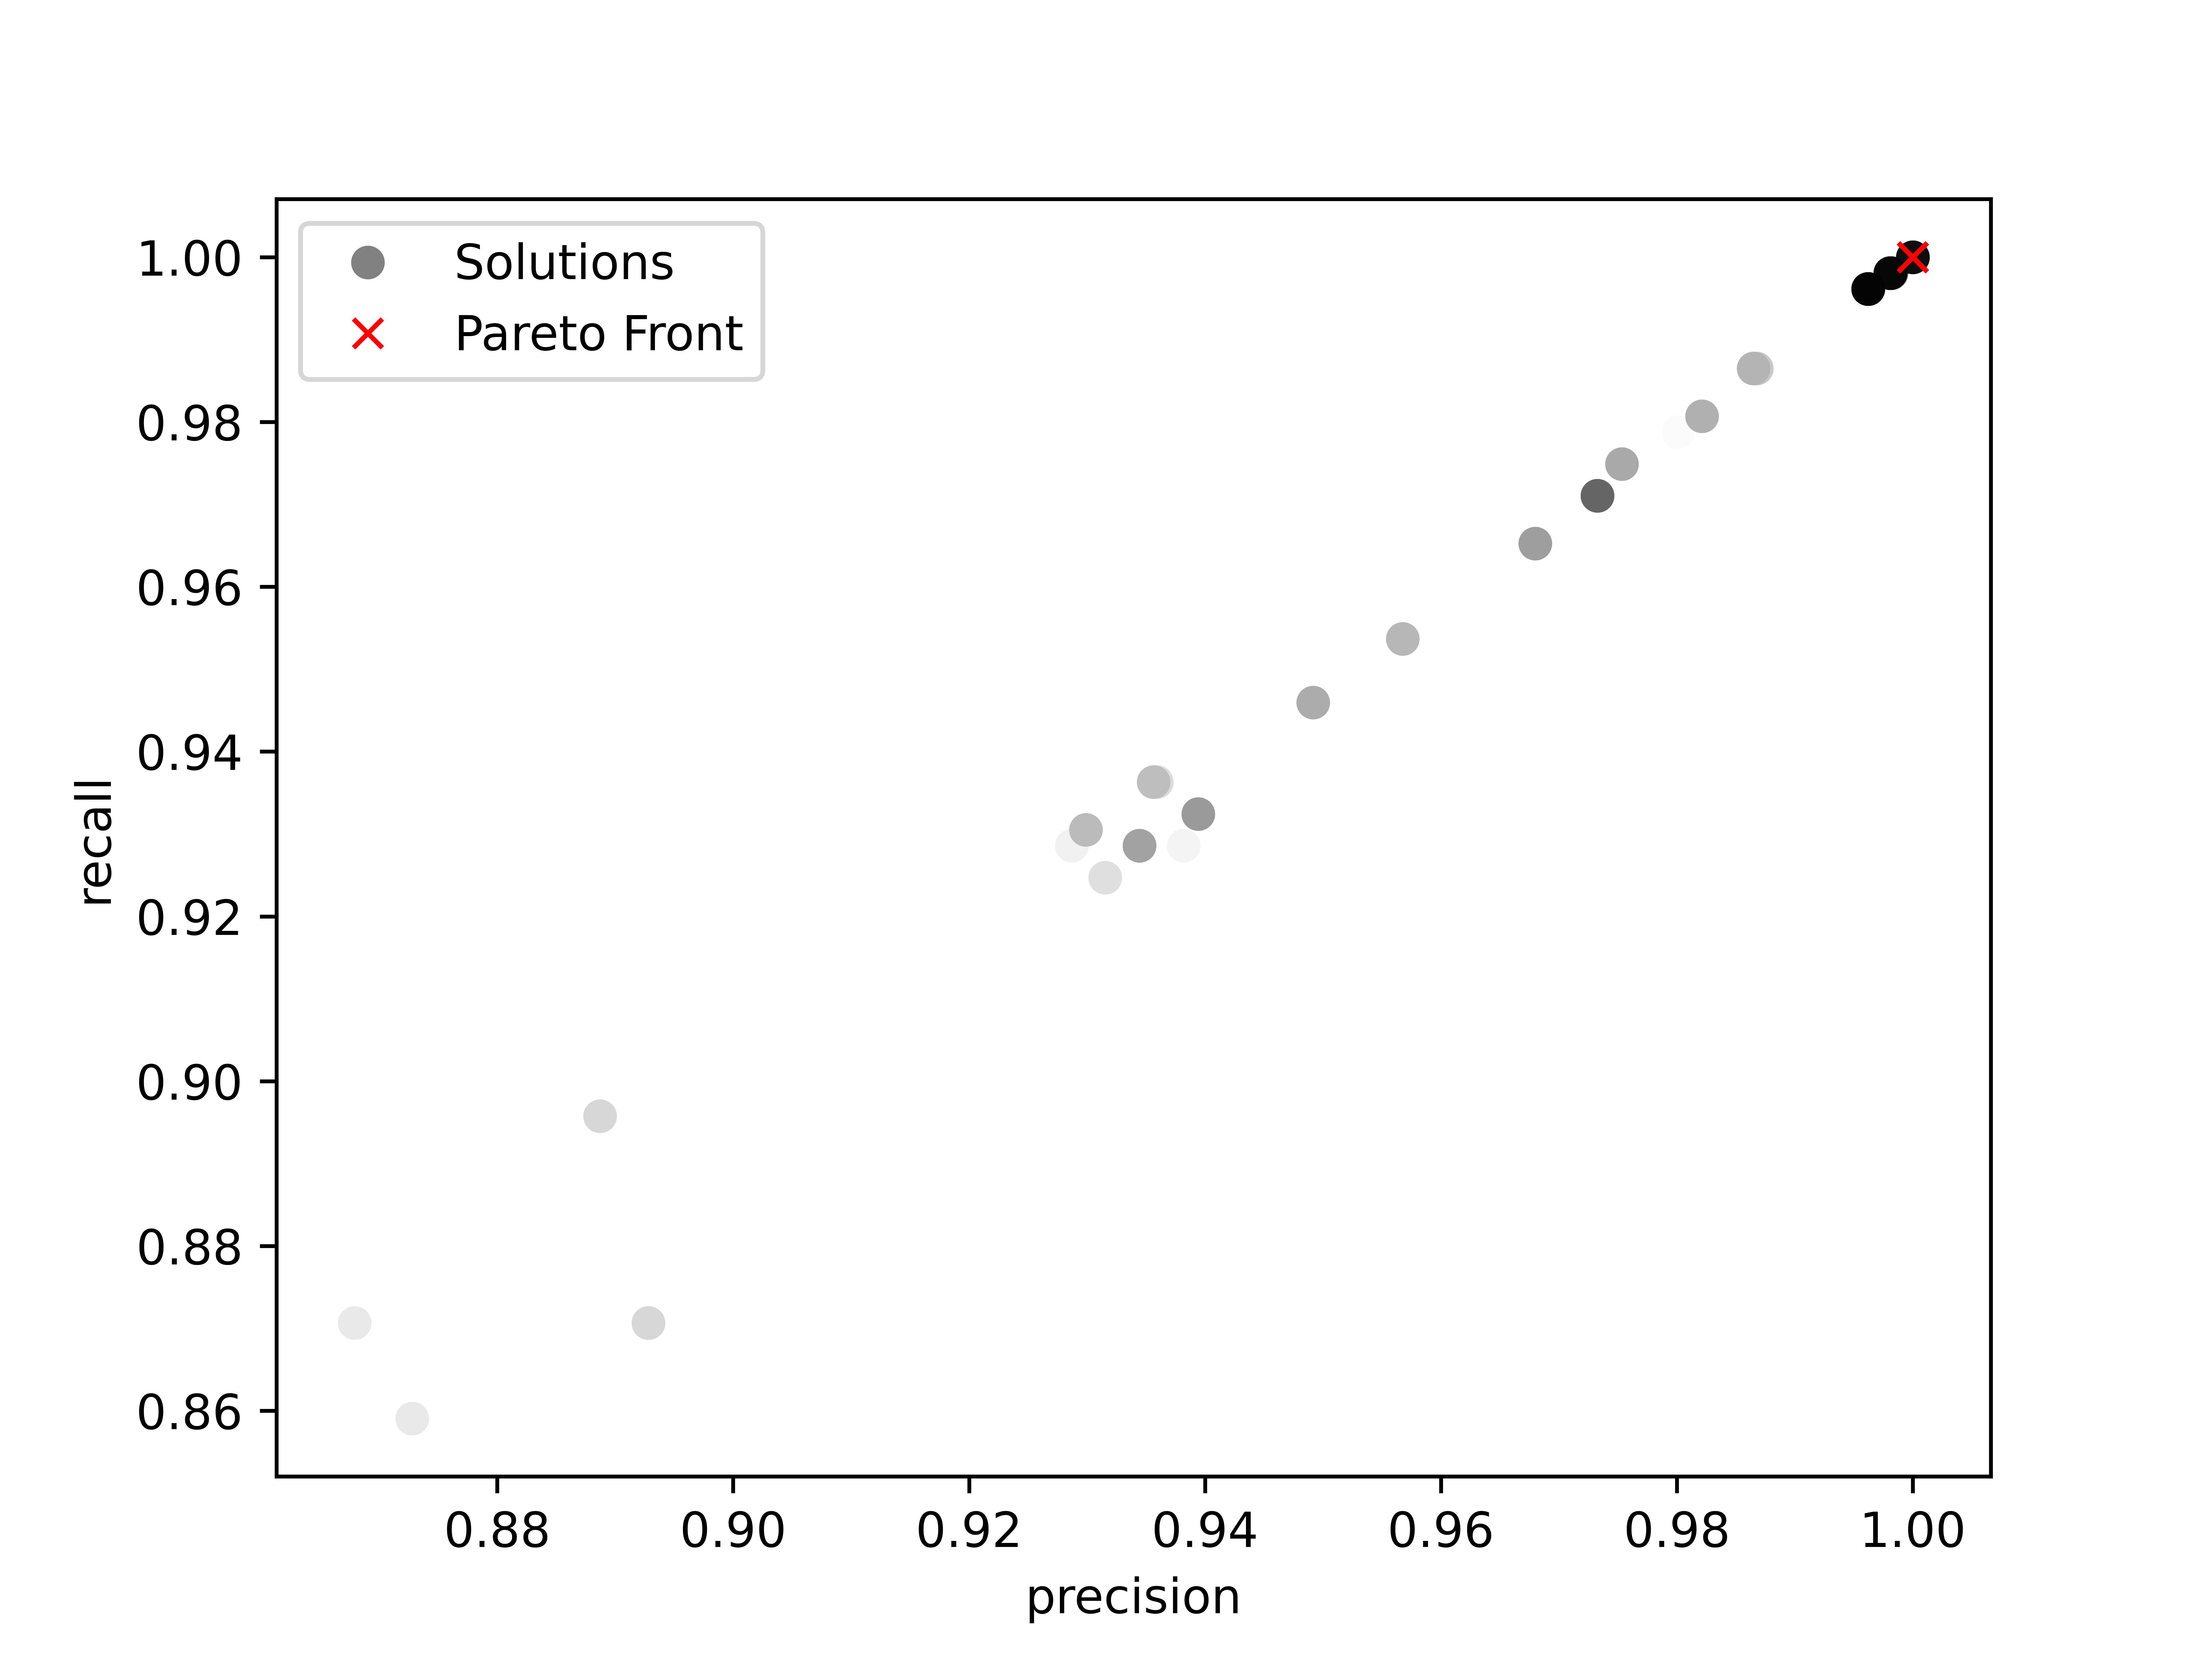
\includegraphics[scale=0.65]{Pictures/cars_precision_vs_recall.jpg}
    \caption{Cars: Precisi\'on contra Recobrado}
    \label{impl:fig:cars:precision_vs_recall}
\end{figure}

\subsection{HAHA}
Se utilizo una poblaci\'on total de 40 individuos, 8 horas de tiempo m\'aximo y 10 segundos por  evaluaci\'on. 
HAHA es un problema de clasificaci\'on binario y las m\'etricas \textit{f-score}, precisi\'on y recobrado son las implementadas en scikit-learn (\cite{pedregosa2011scikit}) utilizando promedio binario.

\subsubsection{F-Score contra Tiempo de Entrenamiento}

En esta prueba el frente obtenido (fig. \ref{impl:fig:haha:fscore_vs_time}) posee una forma aparentemente similar al de Cars (fig. \ref{impl:fig:cars:fscore_vs_time}). Los soluciones de AutoGOAL  est\'an conformados por dos algoritmos principales. Los que contienen una precisi\'on sobre los 0.5 pero son m\'as rapidos est\'an conformados utilizando t\'ecnicas de \textit{Hashing Vectorizer} y \textit{Nearest Centroid} mientras que los de mayor precisi\'on est\'an compuestos por \textit{CountVectorizer}  y regresores log\'isticos.

En la esquina superior izquierda se ve como AutoGOAL busca soluciones que tienen f-score 0, un desperdicio de tiempo de c\'omputo pues el sistema es agn\'ostico al significado de las m\'etricas. Una posible mitigaci\'on a esto es definir no solo las m\'etricas a evaluar si no establecer relaciones entre estas tal como: \textit{if f-score} $== 0 \rightarrow $ \textit{retorna} $-\infty$. Estas restricciones reducen el espacio objetivo y tienen un impacto directo en la b\'usqueda dando a\'un m\'as expresividad a los usuarios de AutoGOAL.

\begin{figure}[ht]
    \centering
    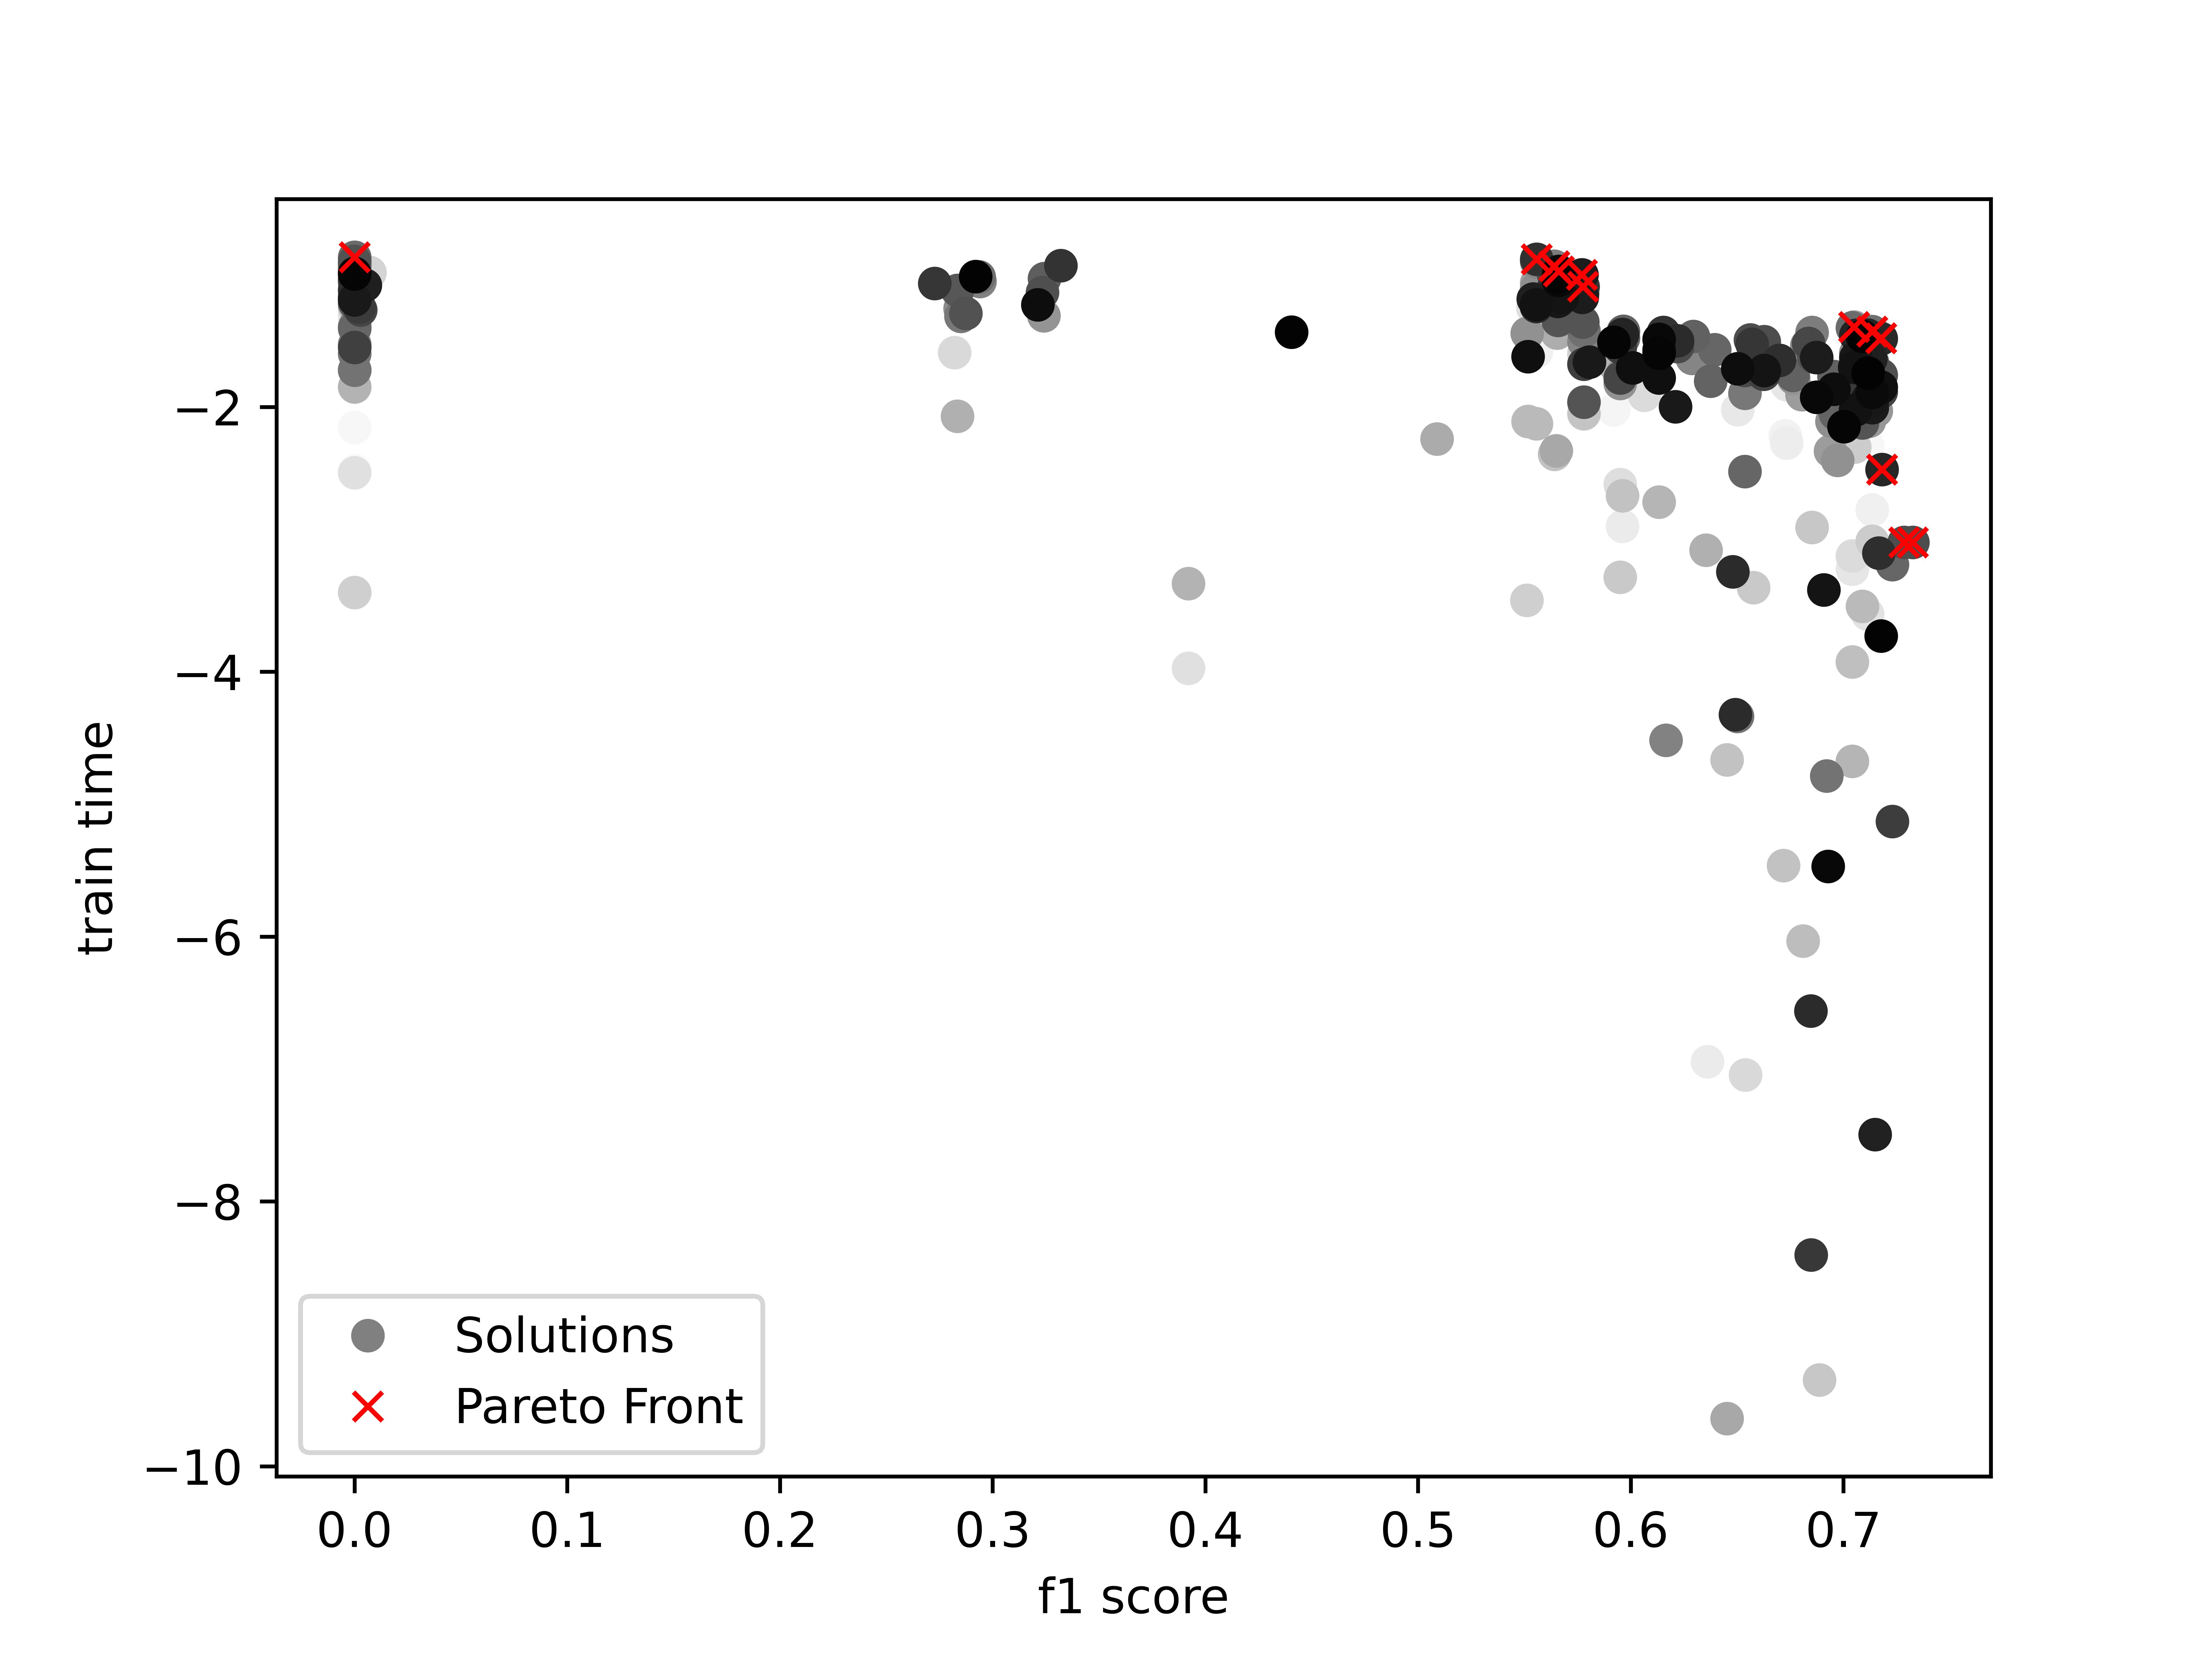
\includegraphics[scale=0.65]{Pictures/haha_fscore_vs_time.jpg}
    \caption{HAHA: F-score contra Tiempo de Entrenamiento (10 segundos m\'ax)}
    \label{impl:fig:haha:fscore_vs_time}
\end{figure}

Otra de las cosas a notar es que hay algoritmos que toman 10 segundos para ejecutarse y posiblemente las soluciones del sistema se vean l\'imitadas por el tiempo m\'aximo asignado a cada \textit{pipeline}. Se realiza una segunda prueba extendiendo esta restricci\'on hasta 3 minutos con el fin de verificar si aumentando el espacio de objetivo se puede obtener una representaci\'on distinta del frente de Pareto. En este caso la estructura extra\~na del frente se mantiene excepto por la aparici\'on de una nueva soluci\'on que destaca sobre el resto con un \textit{f-score} de 0.76 pero con un tiempo de entrenamiento de 31 segundos utilizando un \textit{Count Vectorizer} sin tokenizar y un  clasificador SGD.

\begin{figure}[ht]
    \centering
    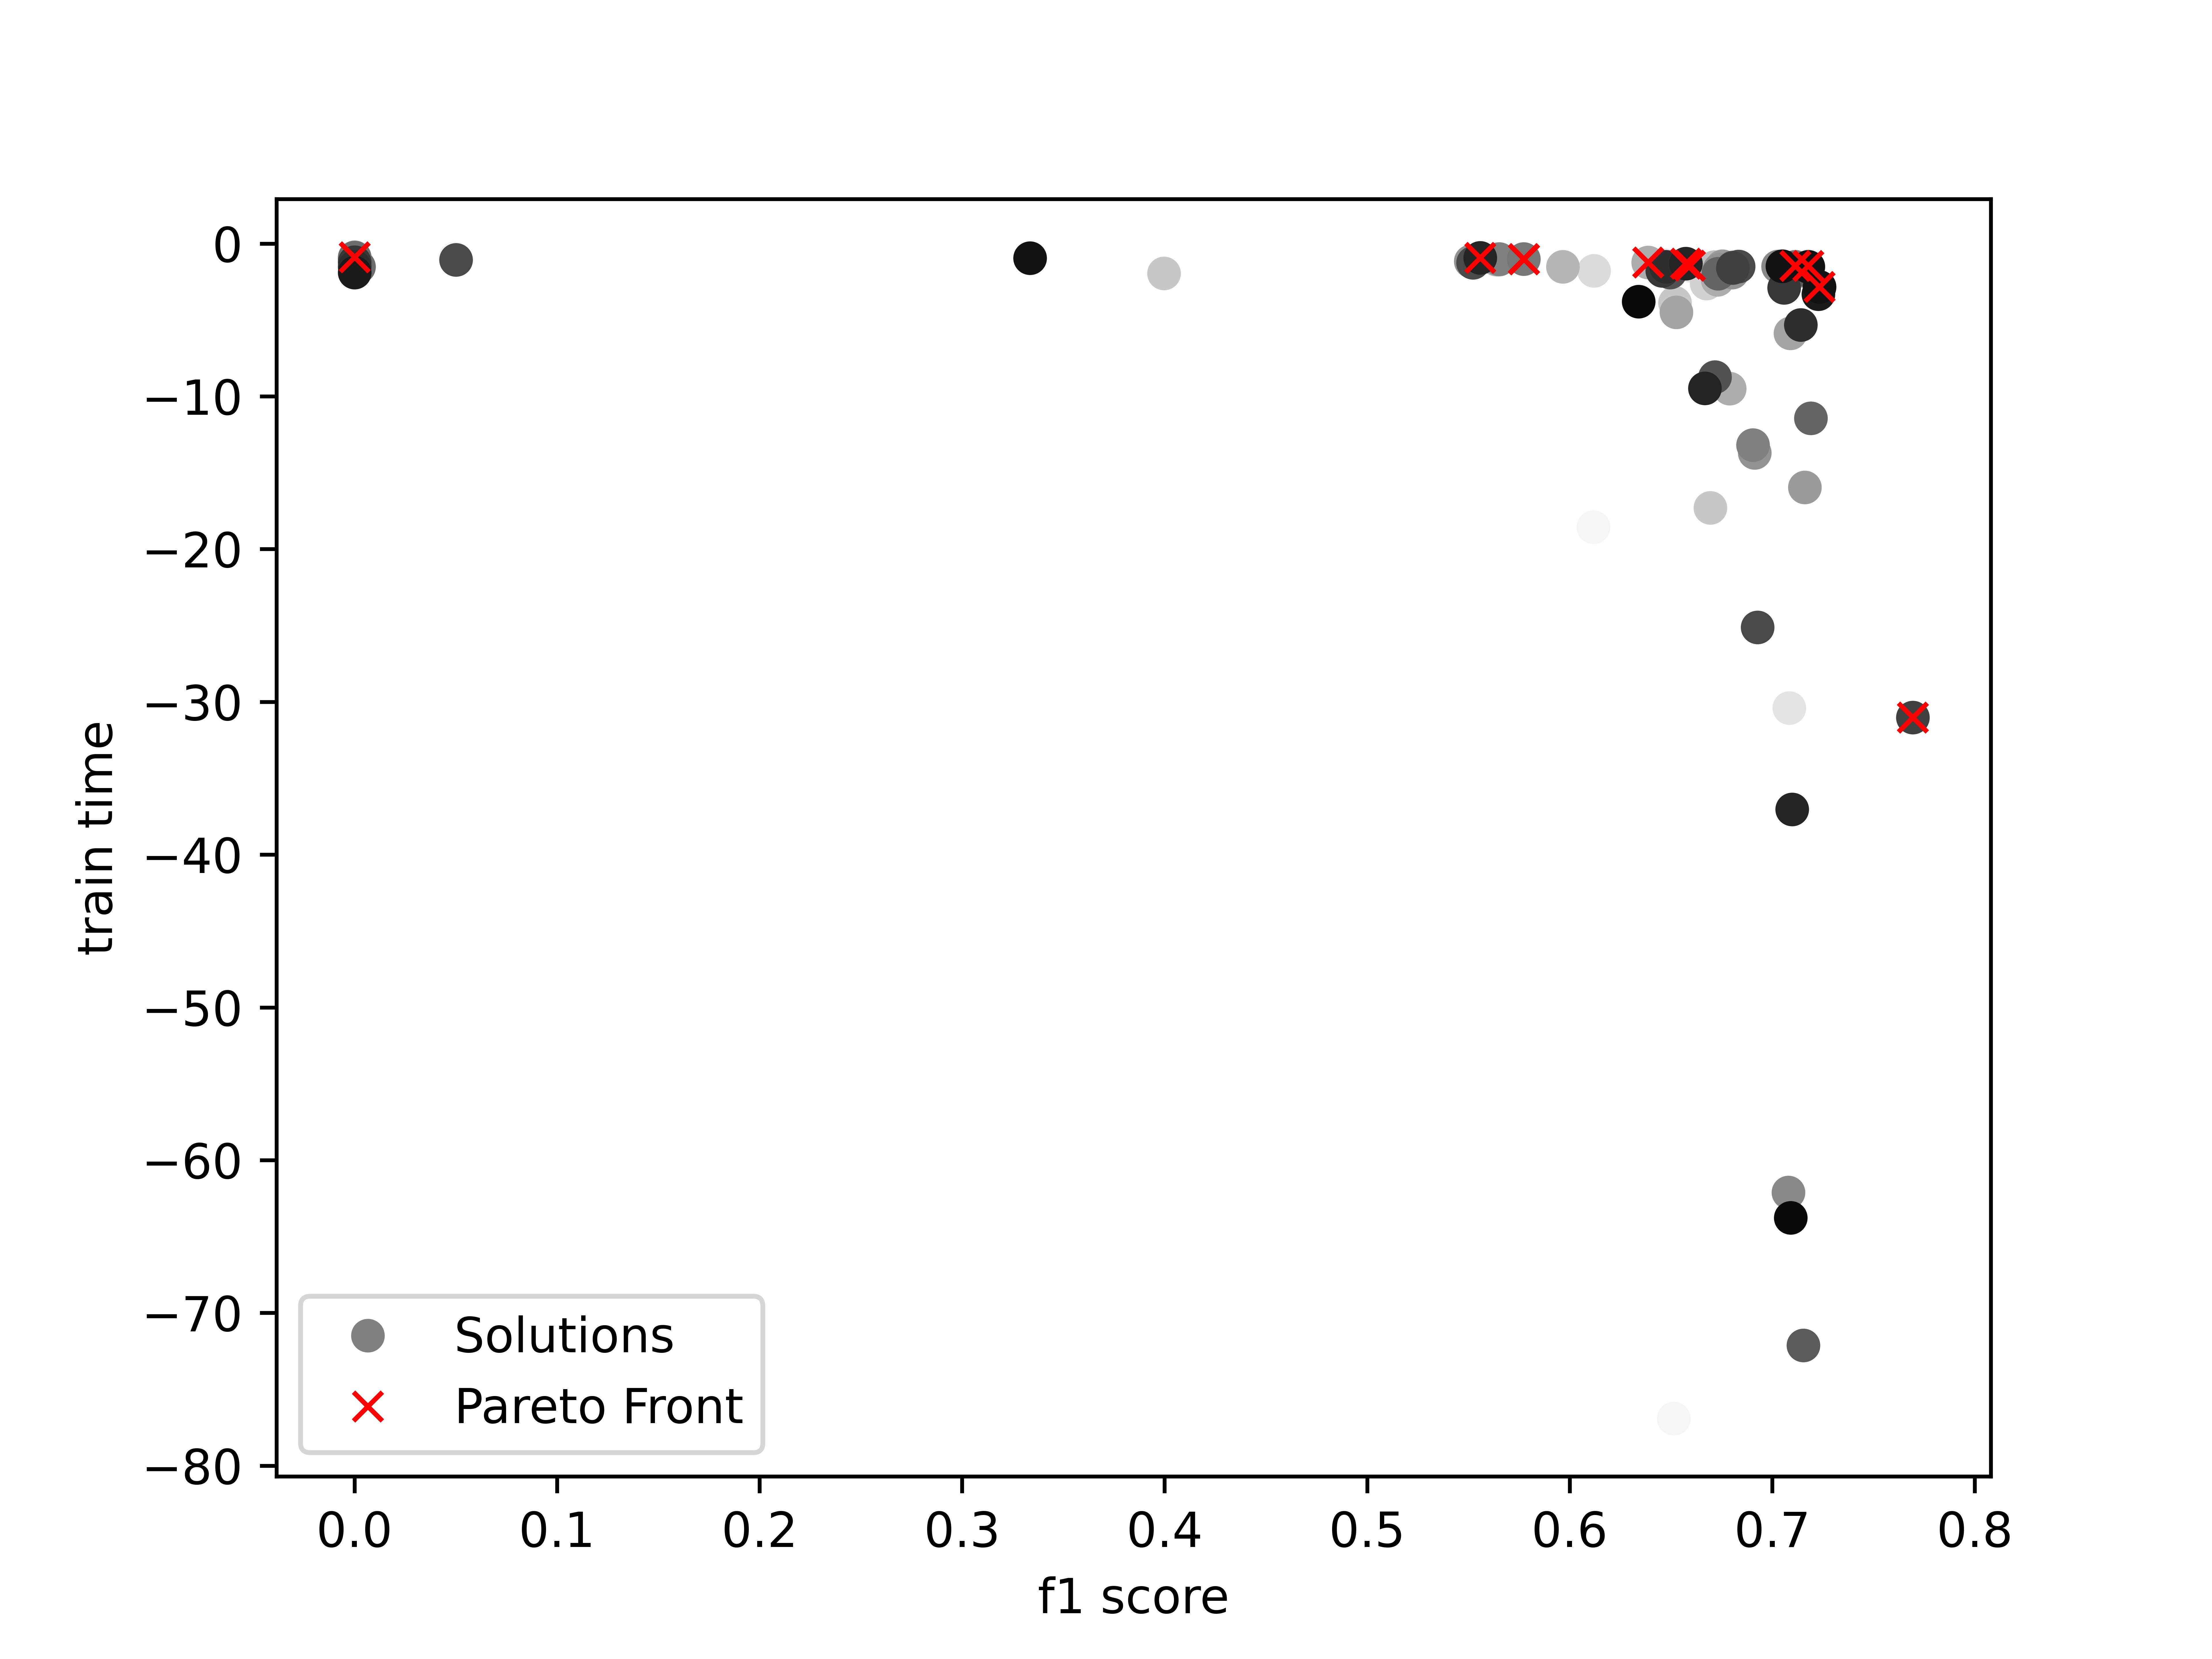
\includegraphics[scale=0.65]{Pictures/haha_fscore_vs_time_3min.jpg}
    \caption{HAHA: F-score contra Tiempo de Entrenamiento (3 minutos m\'ax)}
    \label{impl:fig:haha:fscore_vs_time_3min}
\end{figure}

\subsubsection{Precisi\'on contra Recobrado}
Contrario a lo que muestra la evaluaci\'on de Cars con respecto a precisi\'on y recobrado, durante esta prueba no es posible encontrar un flujo que maximice ambas m\'etricas y es necesario hacer concesiones entre una y la otra. El frente, como se observa en la figura \ref{impl:fig:haha:precision_vs_recall} tiene una forma c\'onvexa, consecuencia del conflicto que se crea al optimizar para estas m\'etricas en este conjunto de datos.

Los flujos obtenidos durante la ejecuci\'on de esta fase presentan mucha mayor diversidad con respecto a todas las pruebas anteriores. Los flujos est\'an compuesto en su mayor\'ia por una tupla de t\'ecnicas de Aprendizaje: un m\'etodo de vectorizaci\'on y un clasificador.

\begin{figure}[ht]
    \centering
    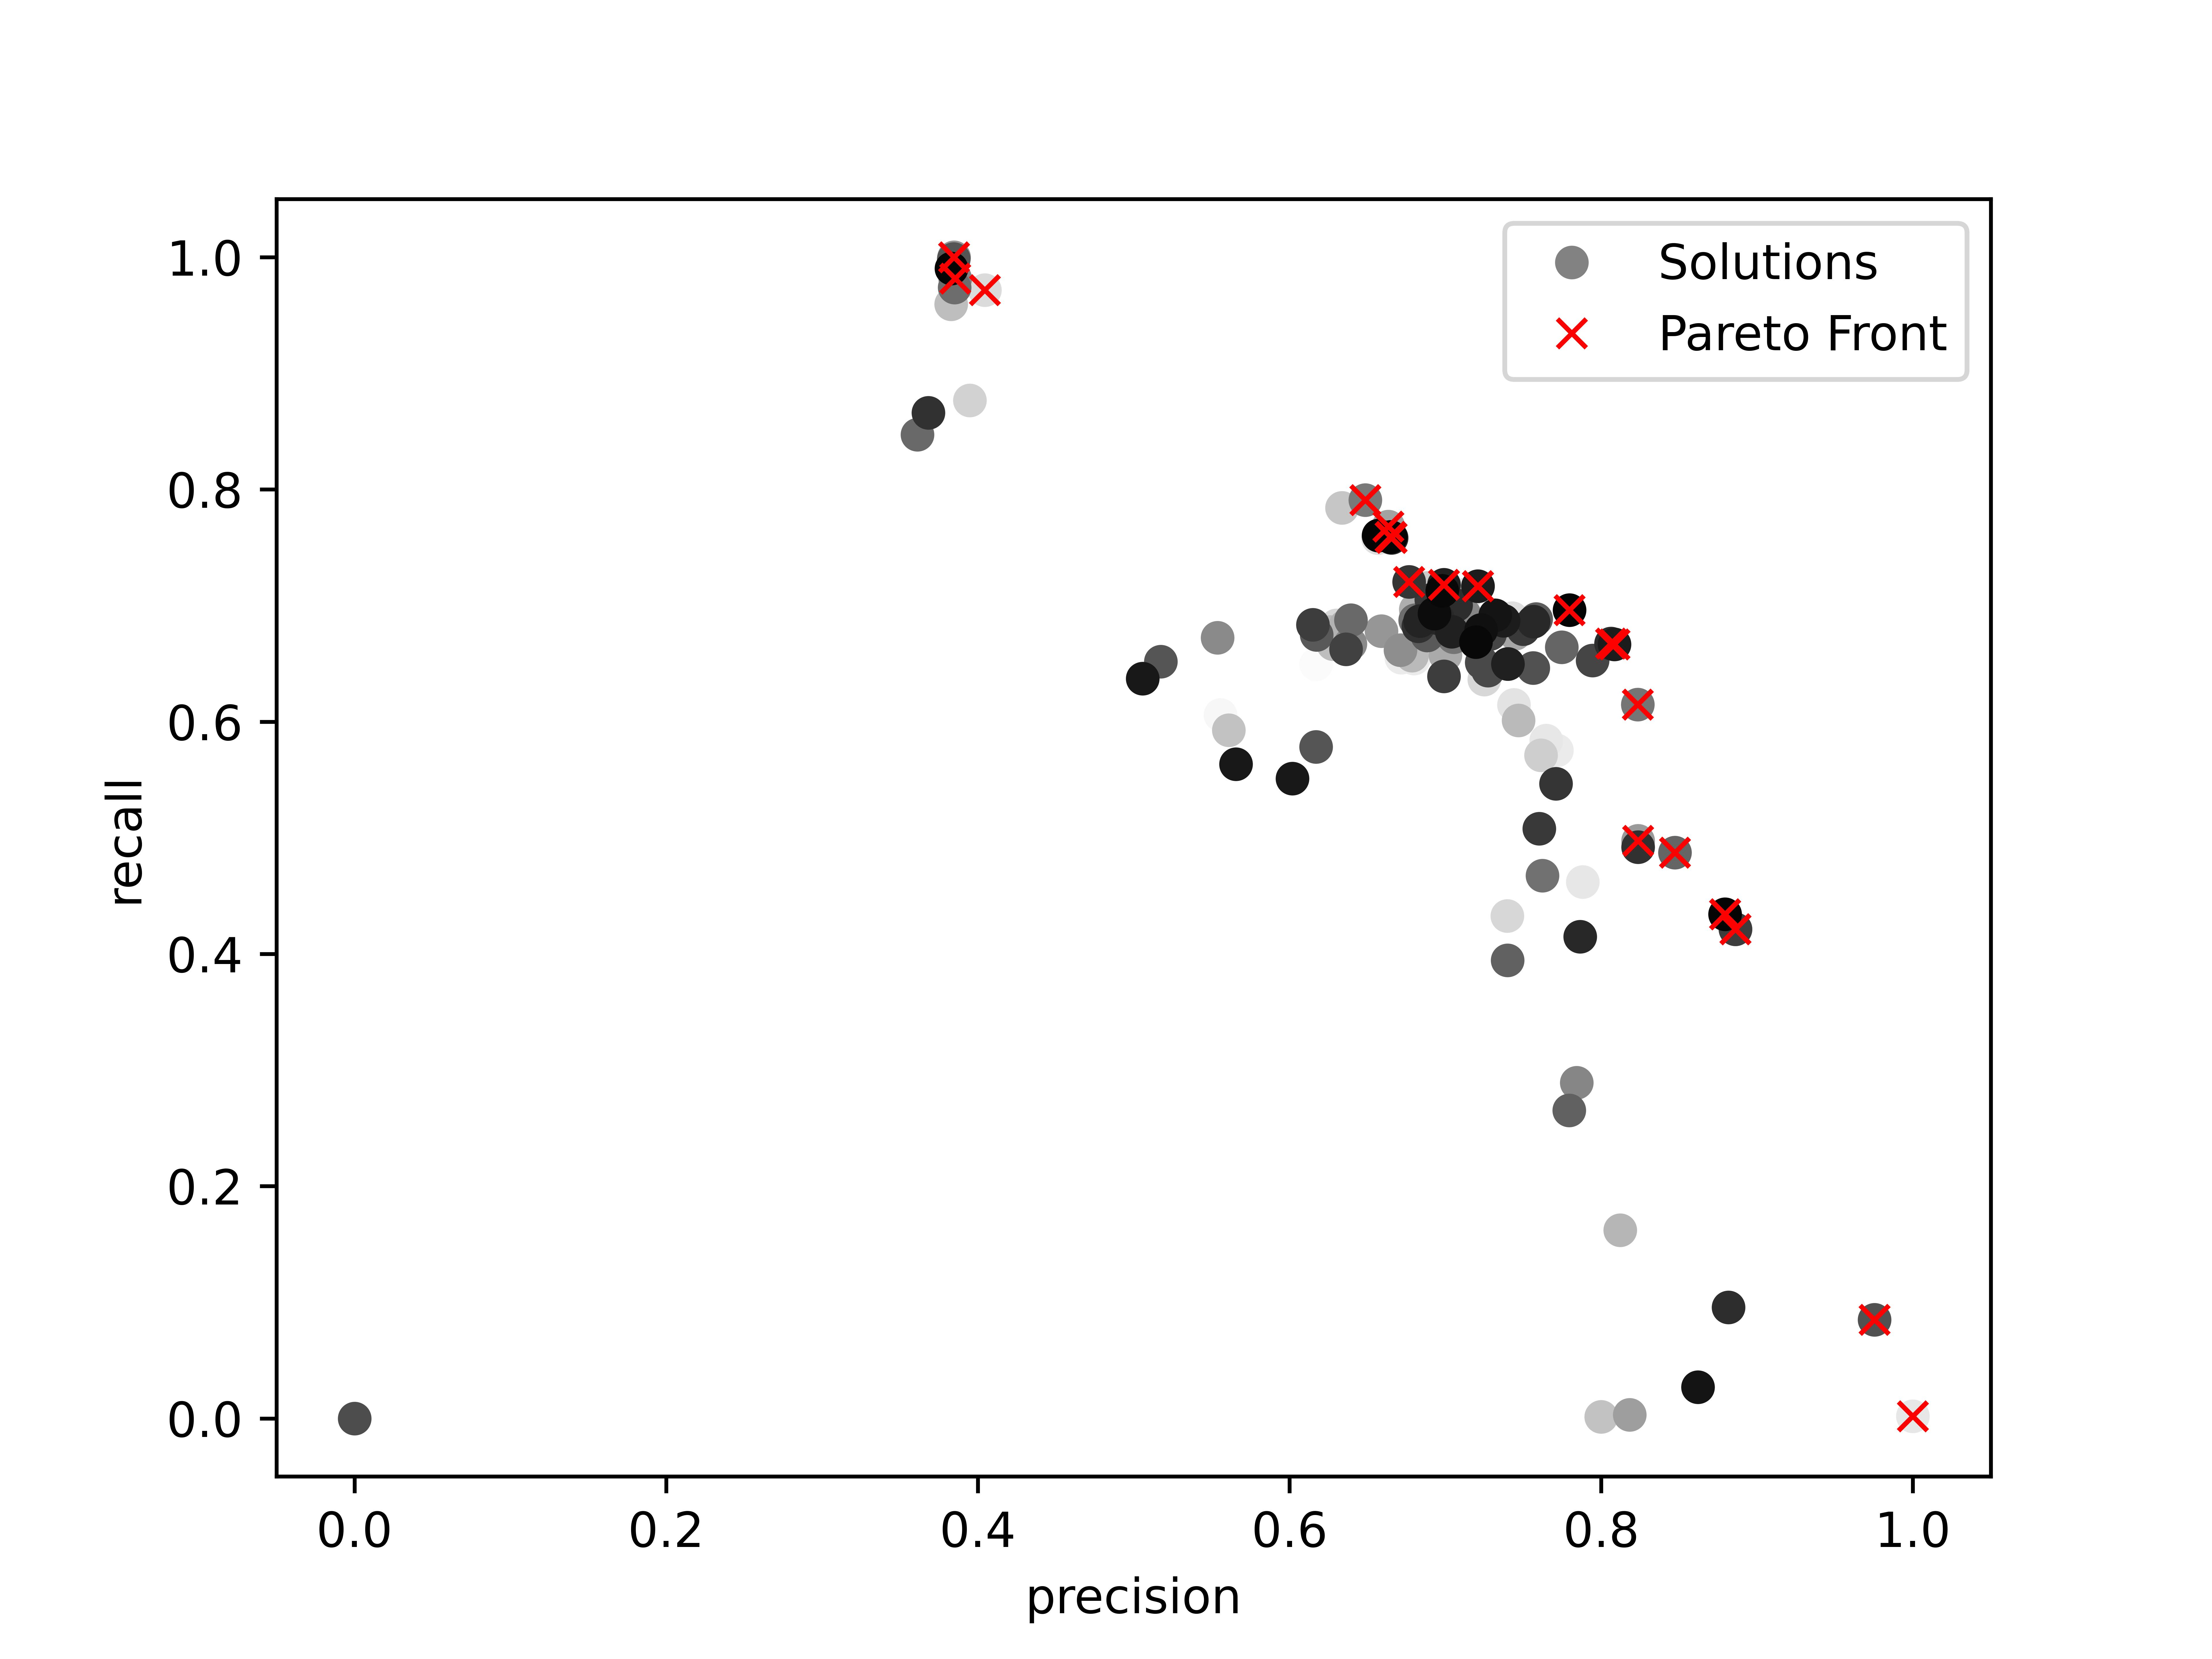
\includegraphics[scale=0.65]{Pictures/haha_precision_vs_recall.jpg}
    \caption{HAHA: Precisi\'on contra Recobrado (10 segundos m\'ax)}
    \label{impl:fig:haha:precision_vs_recall}
\end{figure}

Cuando se optimiza con tiempo m\'aximo de tres minutos (ver figura \ref{impl:fig:haha:precision_vs_recall_3min}) no se muestra ning\'un cambio notable con respecto a la anterior prueba. 

\begin{figure}[ht]
    \centering
    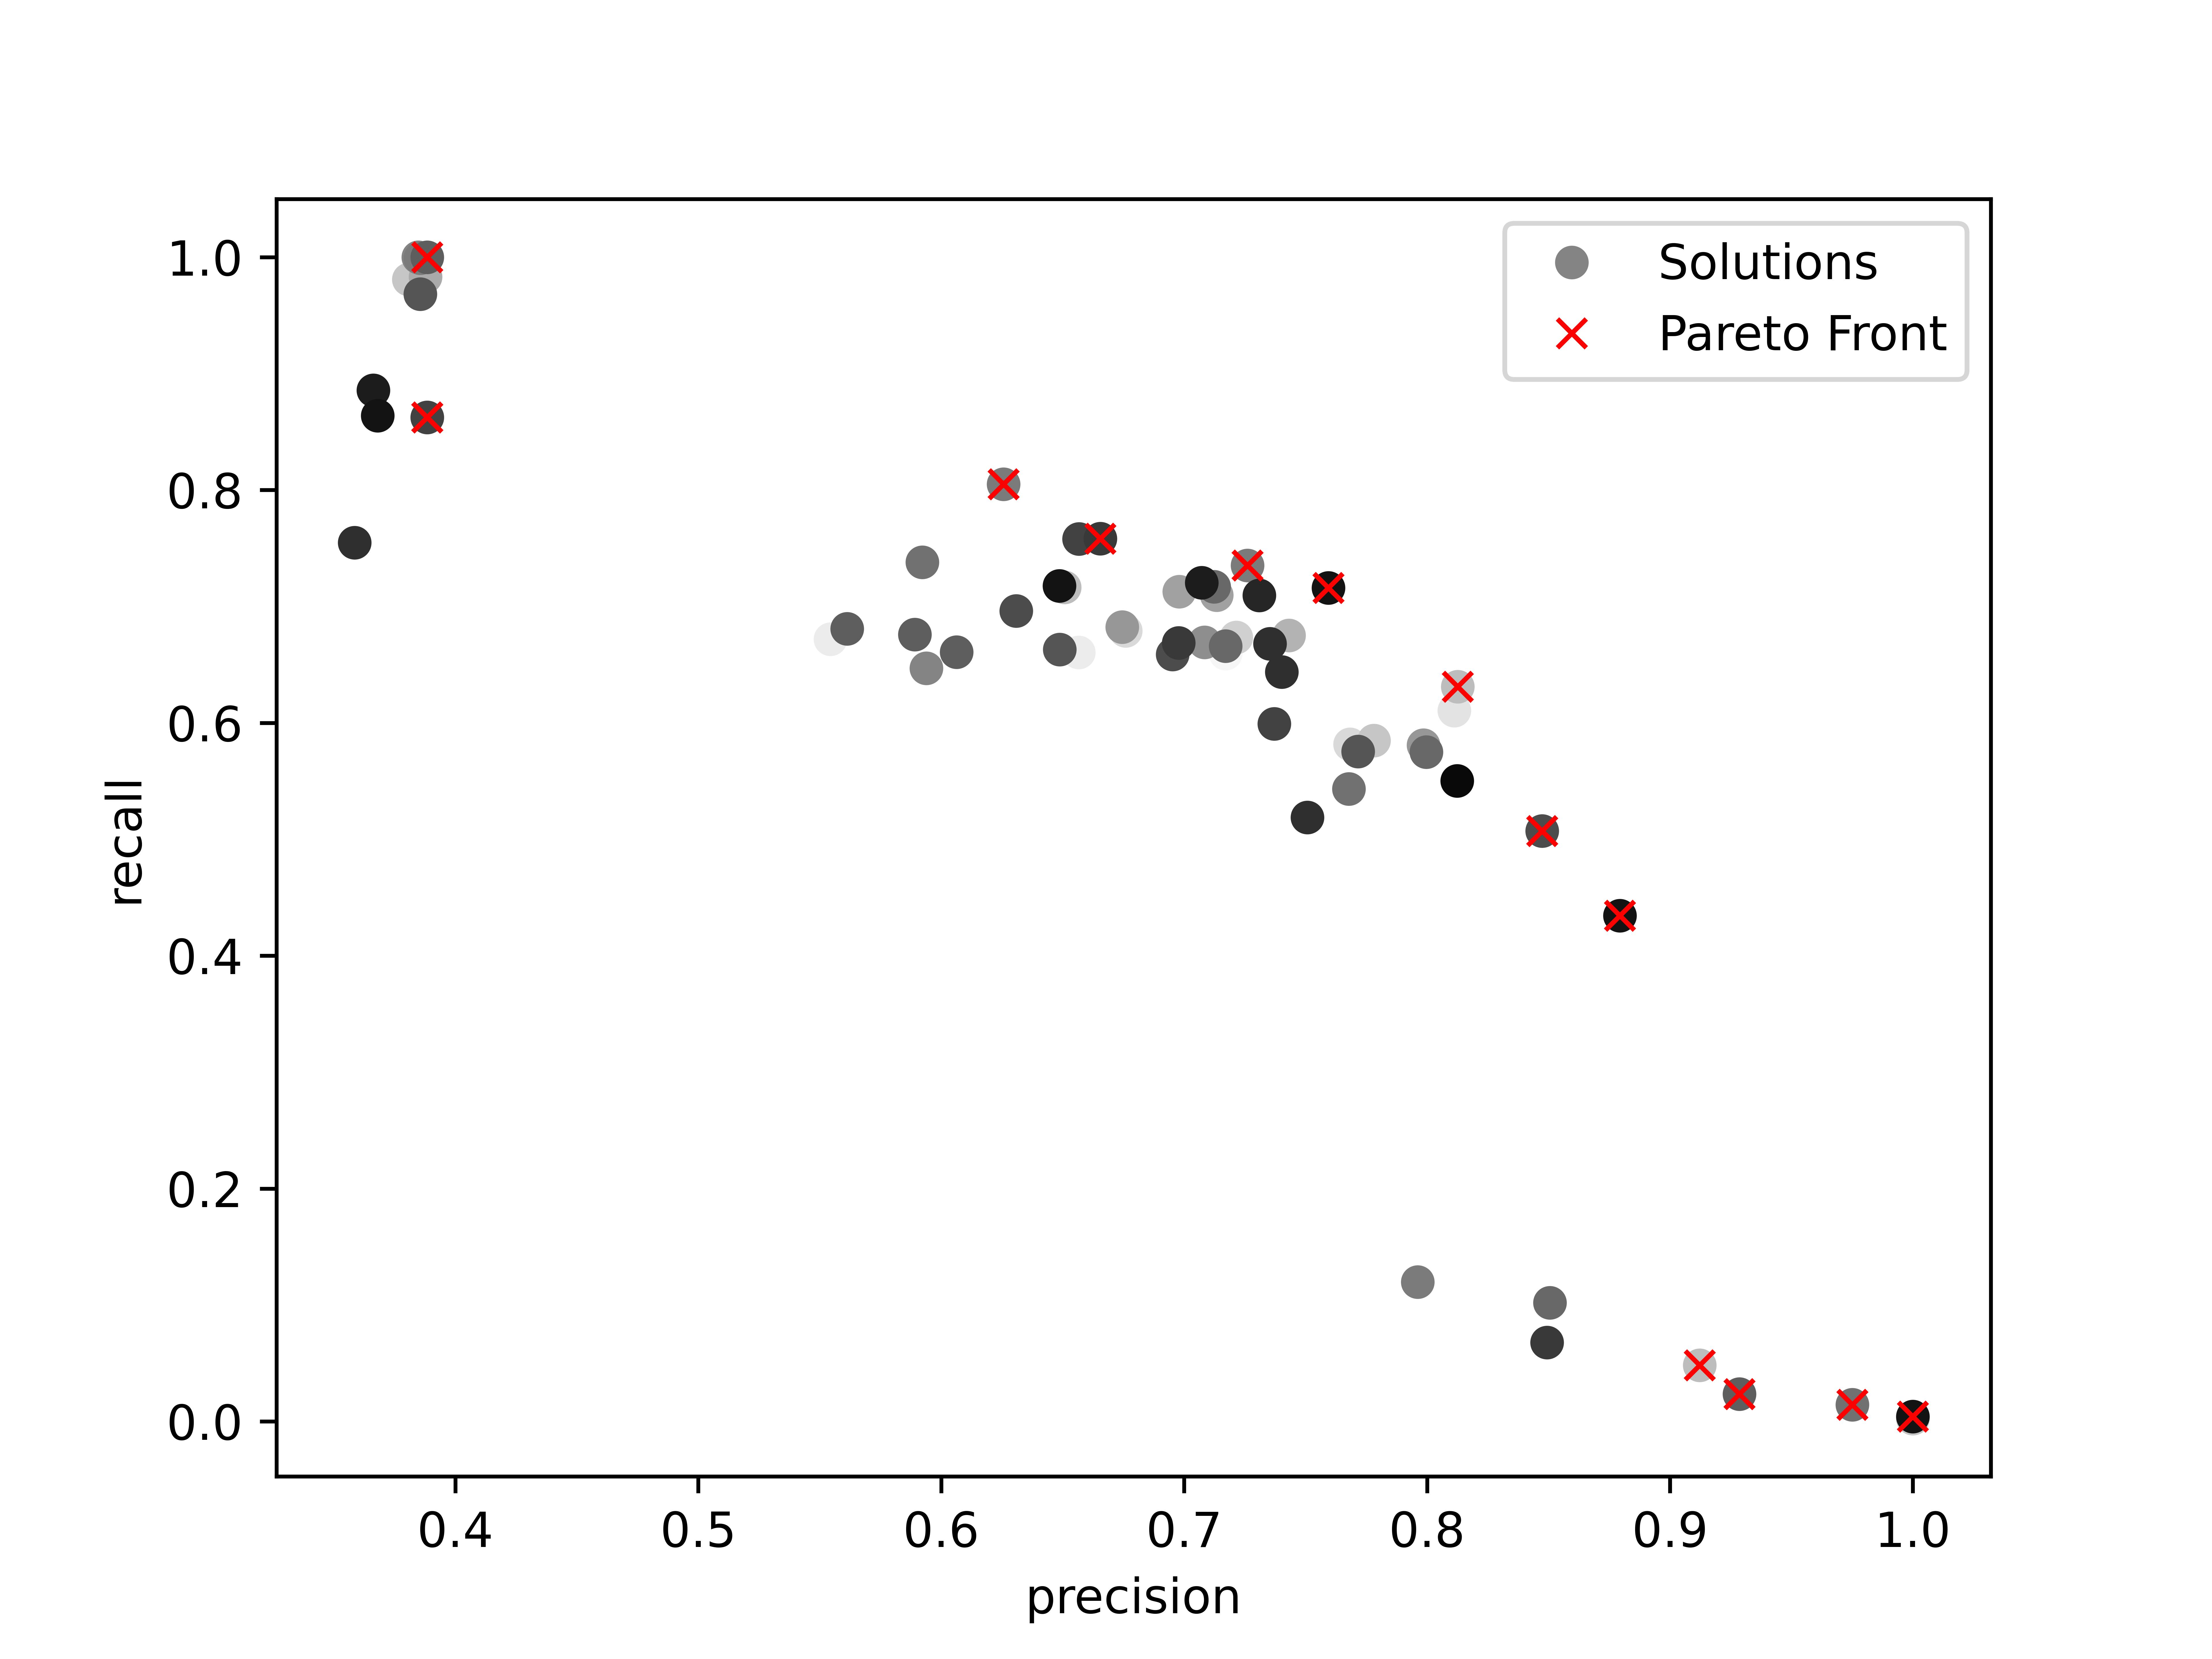
\includegraphics[scale=0.65]{Pictures/haha_precision_vs_recall_3min.jpg}
    \caption{HAHA: Precisi\'on contra Recobrado (3 minutos m\'ax)}
    \label{impl:fig:haha:precision_vs_recall_3min}
\end{figure}

\subsection{MEDDOCAN}
Este corpus representa el conjunto de datos m\'as grande de los tres y  fue necesario aumentar el tiempo de evaluaci\'on por flujo a 10 minutos con el fin de encontrar soluciones v\'alidas, estas tomando tiempos de entre 2 y 6 minutos. Las pruebas fueron ejecutadas con una poblaci\'on total de 50 individuos, 10 horas de tiempo m\'aximo y 10 minutos por evaluaci\'on. 
Las implementaciones de \textit{f-score}, precisi\'on y recobrado son las implementaciones del m\'odulo de Python \textit{meddocan}.
El entrenamiento en esta prueba resultaron ser m\'as lentos y no fue posible realizar muchas iteraciones por lo que no es posible apreciar completamente los frentes.
% Aqu\'i el tiempo m\'aximo es mucho mayor pues es un corpus es mucho m\'as grande que los anteriores que para encontrar al menos un pipeline v\'alido require alrededor de 7 u 8 minutos. Lo suficiente para lograr 3 o 4 generaciones de un total de 100.


\subsubsection{F-Score contra Tiempo de Entrenamiento}
En esta prueba se ve un comportamiento similar a las anteriores como puede observar en la figura  \ref{impl:fig:MEDDOCAN:fscore_vs_train_time} un poco m\'as acentuado en lo que se refiere a m\'etricas de tiempo de entrenamiento pues la diferencia pasa de ser de segundos a minutos. Existe una soluci\'on con un tiempo de 160 segundos y una precisi\'on de 0.83 contra una de 230 segundos y una precisi\'on cercana a 0.9. Existe variedad de t\'ecnicas y tama\~no en los flujos generados .


\begin{figure}[ht]
    \centering
    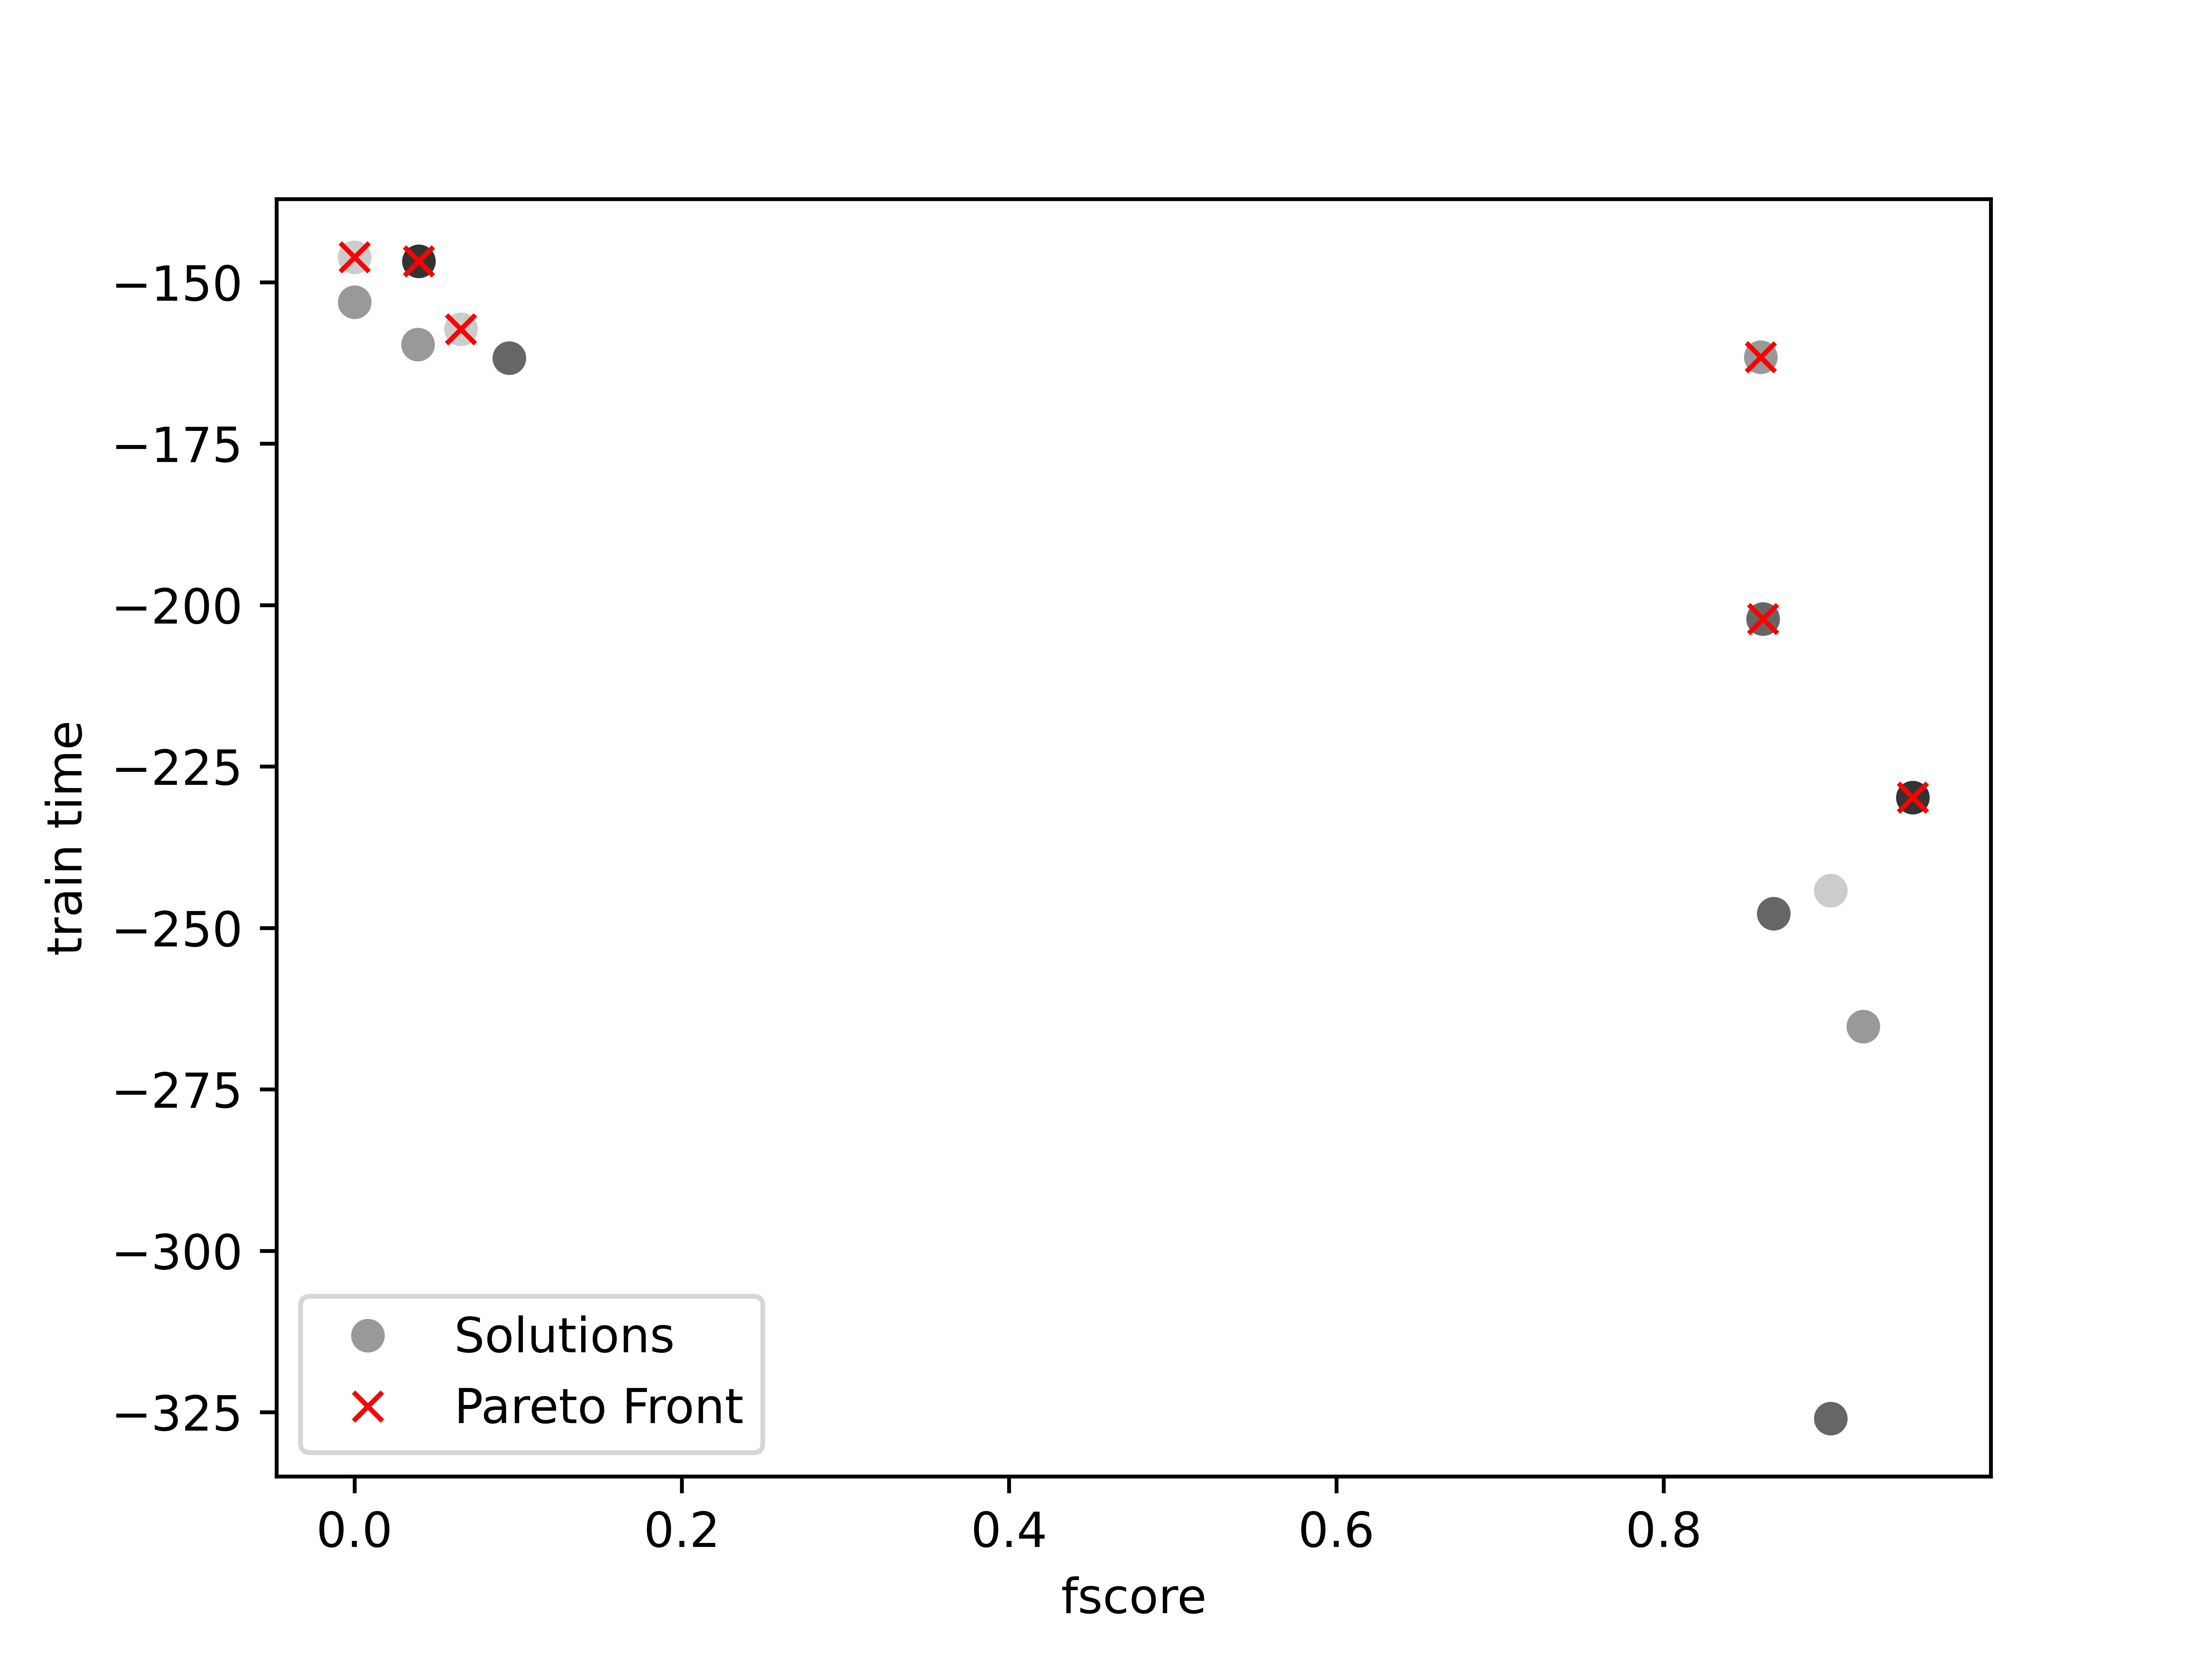
\includegraphics[scale=0.65]{Pictures/meddocan_fscore_vs_train.jpg}
    \caption{MEDDOCAN: F-Score contra Tiempo de Entrenamiento}
    \label{impl:fig:MEDDOCAN:fscore_vs_train_time}
\end{figure}


\subsubsection{Precisi\'on contra Recobrado}
En esta prueba, representada en la figura \ref{impl:fig:MEDDOCAN:precision_vs_recall}, debido a la poca cantidad de iteraciones se obtiene una representaci\'on muy pobre del frente de Pareo. No queda claro si estamos frente a un caso parecido al de precisi\'on contra recobrado de Cars (\ref{impl:fig:cars:precision_vs_recall}) donde las m\'etricas no entran en conflicto y es posible optimizar para ambas, o mas parecido al caso en HAHA (\ref{impl:fig:haha:precision_vs_recall}) donde es obligatorio realizar concesiones.

Un dato interesante de esta prueba en comparaci\'on a cuando se optimiza \textit{f-score} contra tiempo de entrenamiento es que esta realiz\'o menos iteraciones en el mismo rango de tiempo, visible por la diferencia de puntos graficados entre ambas. Esto sugiere que al optimizar utilizando el tiempo como una m\'etrica hace que el sistema priorice flujos r\'apidos de entrenar afectando positivamente la velocidad de b\'usqueda de AutoGOAL.

\begin{figure}[ht]
    \centering
    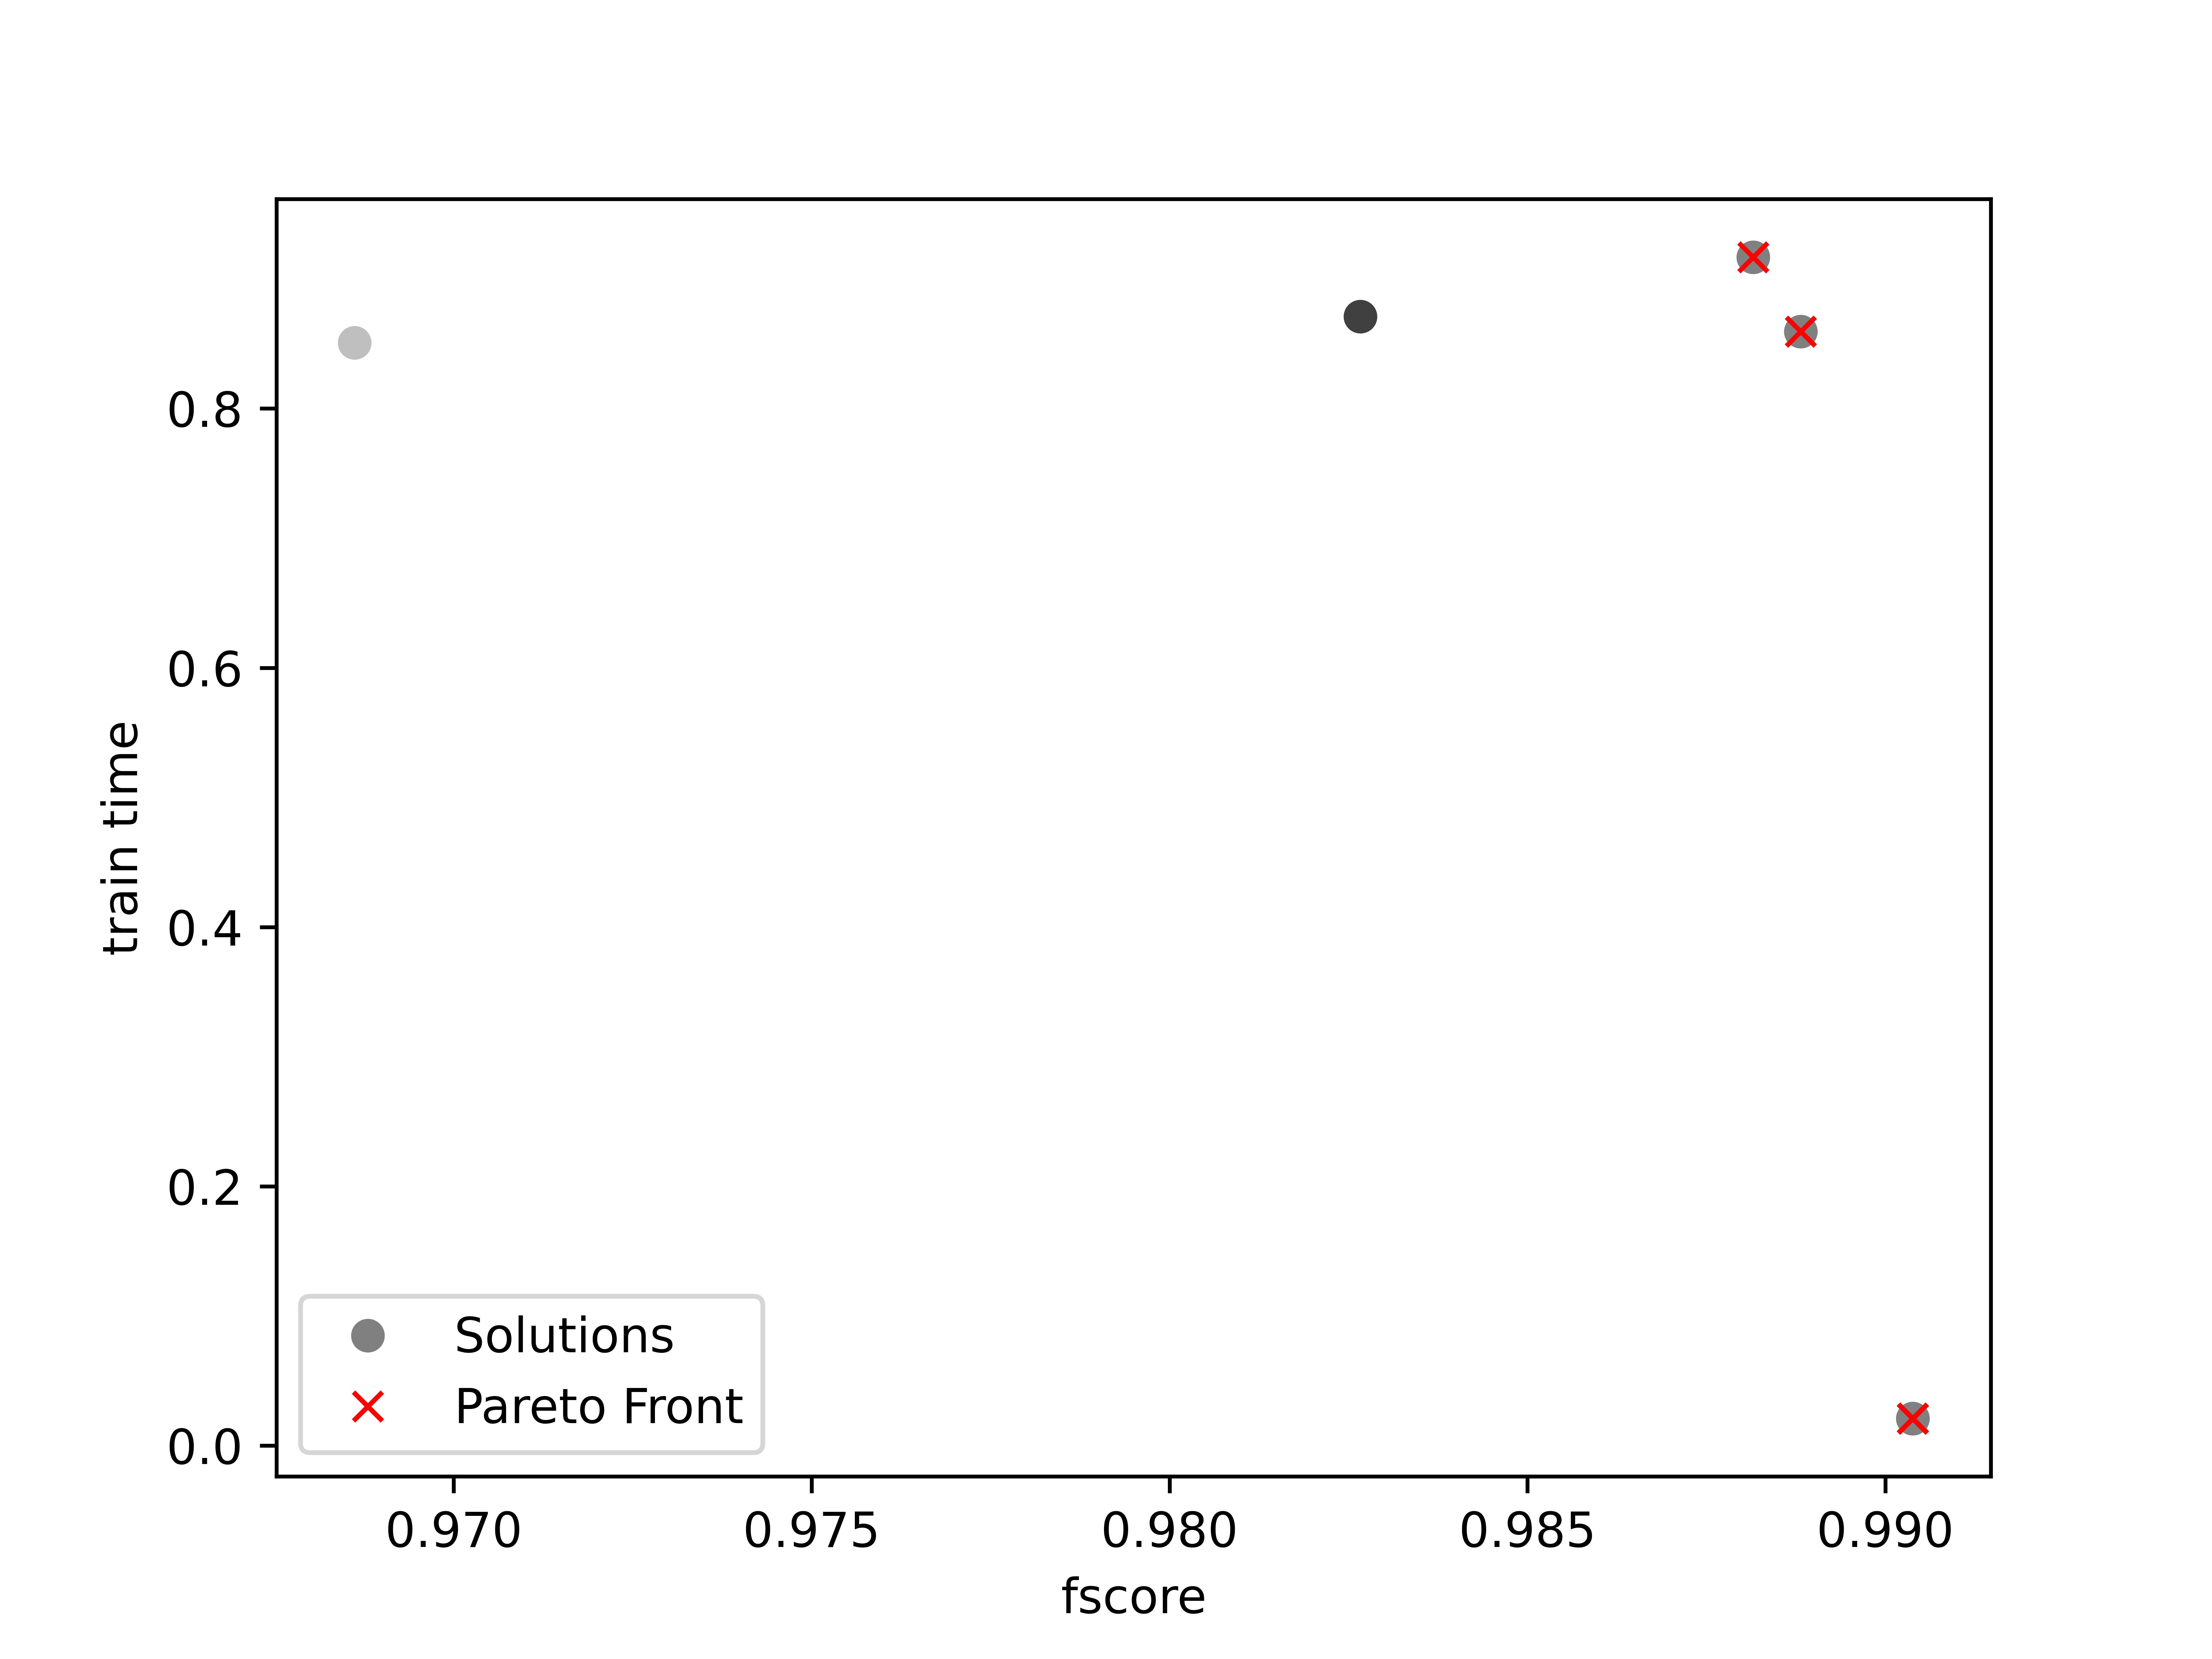
\includegraphics[scale=0.65]{Pictures/meddocan_precision_vs_recall.jpg}
    \caption{MEDDOCAN: Precisi\'on contra Recobrado}
    \label{impl:fig:MEDDOCAN:precision_vs_recall}
\end{figure}


\backmatter

\begin{conclusions}
    Al a\~nadir la habiliad de optimizar en paralelo para muchos objetivos en sistemas AutoML, se crean herramientas que brindan mayor expresivadad a los usuarios permitiendo la soluci\'on y mejoramiento de problemas actuales del campo del Aprendizaje Automatizado como la mitigaci\'on de sesgos. Adem\'as se obtienen beneficios inheretens de la optimizaci\'on multiobjetivo como el retorno de m\'ultples modelos igual de buenos.

    El aprovechamiento de espacios separados donde trabajan las componentes de los sistemas AutoML crea la posiblidad de inclusi\'on de algoritmos multiobjetivos sin ser invasivos sobre los framework ya existentes. Ademas la utilizaci\'on de algoritmos evolutivos multiobjetivo permite la b\'usqueda efectiva de soluciones sobre el frente de Pareto.

    La implementaci\'on basada en AutoGOAL es un ejemplo de cuan f\'acil es adaptar las soluciones ya existentes. La experimentaci\'on utilzando con AutoGOAL muestra resultados prometedores y abren todo un campo de problemas anteriores que se pueden probar nuevamente con esta caracter\'istica. La sencilla intefaz de AutoGOAL se mantiene sin cambios invitando a usuarios de cualquier \'ambito a comprobar esta nueva caracter\'isticas en sus problemas.
Los beneficios que promete la optimziaci\'on multiobjetivo son muchos es cuesti\'on de esperar que sistemas AutoML sigan este curso e implementen optimizaci\'on multiobjetivo.
\end{conclusions}

\begin{recomendations}
Siguiendo la propuesta de AutoML se identifican varias l\'ineas de investigaci\'on y experimentos a realizar para verificar los l\'imites de la propuesta.
\begin{itemize}
    \item Investigar en profundidad en que como la propuesta puede adaptarse a sistemas que no utilizan algoritmos evolutivos para definir su espacio de b\'usqueda tales como los sistemas bayesianos o de aprendizaje por refuerzo.
    \item Replicar las pruebas realizadas en el paper de AutoGOAL utilizando como m\'etrica adicional al tiempo de entrenamiento y comparar las soluciones obtenidas. Verificar si la soluc\'on original de AutoGOAL esta incluida o si se encontraron variantes m\'as veloces. Comprobar que el desempe\~no de las  nuevas variantes  perfomen satisfactoriamente sobre el conjunto de pruebas.
    \item Mejorar el algoritmo multiobjetivo de la propuesta. NSGA-II sufre un defecto caracter\'istico de muchos algoritmos multiobjetivos cuya complejidad computacional crece polinomialmente con el n\'umero de m\'etricas. Es posible mejorar el sistema utilizando algoritmos evolutivos multiobjetivos por descomposic\'on tales como NSGA-III que no sufre de este defecto.
\end{itemize}

\end{recomendations}

\include{BackMatter/Bibliography}

\end{document}
